%%%%%%%%%%%%%%%%%%%%%%%%%%%%%%%%%%%%%%%%%%%%%%%%%%%%%%%%%%%%%%%%%%%%%%%%%%%%%%%%
%
%   Semester project, fall term 2014
%   Author: Jakob Ehrl, born 01/24/91
%   Study program: Computer science, MA 1
%   
%   Professor Dr. Francesco Mondada
%   Assistant: Dr. Stefan Witwicki
%
%%%%%%%%%%%%%%%%%%%%%%%%%%%%%%%%%%%%%%%%%%%%%%%%%%%%%%%%%%%%%%%%%%%%%%%%%%%%%%%%%

%%%%%%%%%%%%%%%%%%%%%%%%%%%%%%%%%%%%%%%%%%%%%%%%%%%%%%%%%%%%%%%%%%%%%%%%%%%%%%%%
%
%   Semester project, fall term 2014
%   Author: Jakob Ehrl, born 01/24/91
%   Study program: Computer science, MA 1
%   
%   Professor Dr. Francesco Mondada
%   Assistant: Dr. Stefan Witwicki
%
%%%%%%%%%%%%%%%%%%%%%%%%%%%%%%%%%%%%%%%%%%%%%%%%%%%%%%%%%%%%%%%%%%%%%%%%%%%%%%%%%

\documentclass[english,rep]{lmedoc}

%\usepackage[latin1]{inputenc}
\usepackage{pdfpages}
\usepackage{tabularx}
\usepackage{subfigure}
\usepackage{color}
\usepackage{pgfplots}

% algorithms
\usepackage[]{algorithm}
\usepackage[]{algpseudocode}

% code listings
\usepackage{listings}
\usepackage{xcolor}

% specific settings
\hbadness=10000
\pagenumbering{roman}
\bibliographystyle{galpha1a}

% for tikz plots:
\pgfplotsset{
	compat=1.8,
	height=0.3\textheight,
	width=0.5\textwidth-5pt,
	legend columns={2},
}
\usepgfplotslibrary{external}
\usetikzlibrary{calc}
\tikzexternalize%activate externalization!
\usepackage{wrapfig}

\graphicspath{ {figures/} }

\pgfplotscreateplotcyclelist{system-plots}{
red,
blue,
orange,
cyan
}

% for code listings
\definecolor{dkgreen}{rgb}{0,0.6,0}
\definecolor{gray}{rgb}{0.5,0.5,0.5}
\definecolor{mauve}{rgb}{0.58,0,0.82}

\lstset{
frame=tb,
%language=scala,
aboveskip=3mm,
belowskip=3mm,
showstringspaces=false,
columns=flexible,
basicstyle={\small\ttfamily},
numbers=none,
numberstyle=\tiny\color{gray},
keywordstyle=\color{blue},
commentstyle=\color{dkgreen},
stringstyle=\color{mauve},
breaklines=true,
breakatwhitespace=true,
tabsize=3,
}



\includeonly{rc01, rc02, rc03, rc04, rc05, rc06, rc07, rc-lit, rc-lof, rc-lot}

\begin{document}

\clearpage
  \begin{deckblatt}
    \Titel{STI Robot competition}
    \NameA{Ehrl}
    \VornameA{Jakob}
    \NameB{Longobardi}
    \VornameB{Pasquale}
    \NameC{Unnervik}
    \VornameC{Eric}
   \Betreuer{Tomasz Gorecki}
    \Start{February 22nd 2015}
    \Ende{June 5th 2015}
  \end{deckblatt}

%\cleardoublepage


\begin{center}
\bfseries
Abstract
\normalfont
\end{center}
This report presents in detail the phases that have brought to the realization of a mobile, autonomous robot conceived to participate to the STI Robot Competition 2015 . This competition aims to allow student at master level to come up with solutions, for a recycling robot for PET bottles collection and transport in a reserved area, dealing with the difficulties coming from a challenging environment such as complex terrains and obtacles. The participation to this competition, as fulfillment of the master’s semester project for our team, involved the complete design of the robotic system in every aspect from hardware to software allowing us to face all the usual challenges that are encountered through the achievement of such a project. The design of the mechanical parts has been coupled with the choice of sensors and actuators exploited by developing algorithms in order to achieve perception, actuation, navigation and localization tasks that gave to the robot the necessary skills to take part in the competition.

%\cleardoublepage
\clearpage

\tableofcontents

%\cleardoublepage
\clearpage

\pagenumbering{arabic}

%%%%%%%%%%%%%%%%%%%%%%%%%%%%%%%%%%%%%%%%%%%%%%%%%%%%%%%%%%%%%%%%%%%%%%%%%%%%%%%%
%
%   Semester project, fall term 2014
%   Author: Jakob Ehrl, born 01/24/91
%   Study program: Computer science, MA 1
%   
%   Professor Dr. Francesco Mondada
%   Assistant: Dr. Stefan Witwicki
%
%%%%%%%%%%%%%%%%%%%%%%%%%%%%%%%%%%%%%%%%%%%%%%%%%%%%%%%%%%%%%%%%%%%%%%%%%%%%%%%%%

\chapter{Introduction}

\section{Description of the challenge}
This competition involves 5 teams of 3 students coming from different sections and aims to challenge the students in building  an autonomous mobile robot for PET bottles collection and transport in a reserved area.
In the figure below (Figure \ref{fig:Arena}) is represented the 8mx8m arena where the robot will have to work.
The arena is divided in 4 differents zones and, according to the difficulty to access or to perform in the zone, and the weight in terms of points accorded for each bottle collected is different.

\begin{figure}[H]
  \centering
  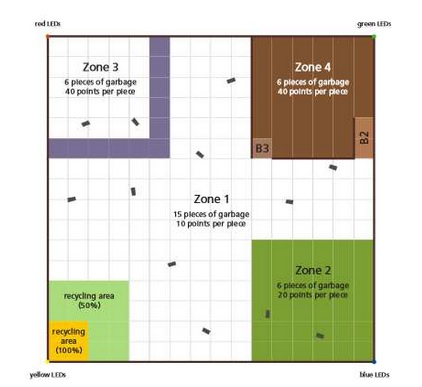
\includegraphics[width=0.6\textwidth]{Arena.jpg}
  \caption{Arena configuration.}
\label{fig:Arena}
\end{figure}

After being picked up the PET bottles need to be transported to a 1mx1m recycling area (left-down corner in Figure \ref{fig:Arena}) in order to be awarded with the 100\% of the points given by the bottles.
If they were to be released within the second limit of the recycling area they would be worth 50\% of the points. Finally if they were to be kept within the robot the amounts in points would be 25\% of the actual value of the collected bottle. 

%\chapter{Research}

%\section{Ideas}
%some drawings and stuff from the main ideas in the %beginning

\section{Selection process}

%(The tables where we chose the features of the robot, and the cahier des charges that we should respect)

Firstly, as a group, we evaluated all the possible strategies that could lead to the achievement of the goal.
In the following, can be found in a schematic way the charts describing the morphology of all the solutions that have been evaluated as well as the choices that brought us to the final design of our robot that will be treated in the following section.

This first chart (Figure \ref{fig:MechanicalChoices}) analyzes the possible solutions that we evaluated for the robot's locomotion. In particular, the wheeled solutions, refer to the use of the Wild thumper chassis that can be modified exploiting either 4 or 6 wheels. The Wild thumper chassis is easy to modify, add components to, since it has holes in it, and is a rather modular chassis, that can be modified, and decomposed into smaller parts. This chassis was the one present in the catalogue, therefore the easiest to obtain. Furthermore this kind of structure had been used also in the previous editions of the competition and this was a good basis in terms of experience to begin with. A custom chassis was also possible to obtain, since workshops were available to manufacture parts for the competition, however, the workload was already very high, and the workshops were already very busy and could only manufacture a very limited number of parts.
Others solutions like rubber tracks and swedish wheels have also been evaluated. However, as depicted in the related chart, the advantages in using the Wild Thumper chassis with 4 wheels resulted more appealing to us, in particular its polyvalence, making us pick up this solution for the robot’s locomotion.

\begin{figure}[H]
 \centering
 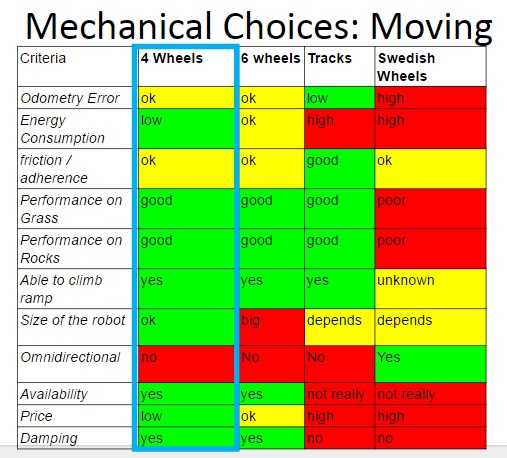
\includegraphics[width=0.7\textwidth]{MechanicalChoises.jpg}
 \caption{Morphological chart of the mechanical criteria.}
\label{fig:MechanicalChoices}
\end{figure}

The objective of the competition was the collection of bottles, so right after choosing the locomotion method we started evaluating the possible solutions to accomplish this goal.
The first evaluation we made has been about the principle behind the system.
Indeed there are two possible approaches to the achievement of this task:

\begin{itemize}
\item Selective Approach
\item Greedy Approach
\end{itemize}

In a selective approach, each bottle has to be detected and, furthermore, its position and orientation need to be computed in order to approach the PET bottle in the desired way and grasping it by mean of a robotic arm or another precise pick up system (see the solution of group 3). 
However, this kind of solution, even if fascinating, appeared to us as a constraint and would have inevitably led to a too high workload. 
As the duration of the competition was only 10 minutes, we assumed that a selective approach was too slow to pick up many bottles in such a short time. Thus we pointed toward a more greedy approach.
In a greedy approach, bottles don’t need to be perfectly identified and they could be picked up also by only being in the path of the robot.
With this idea in mind we started evaluating the mechanic systems that could provide such a favorable behavior.
The evaluated solutions are shown in the chart in Figure \ref{fig:PickUpApproach}.
In our case we have chosen to couple a rigid elevator, which aims to pick up the bottle from the terrain putting it in a storage area upon the robot, with a rotating sponge, as the ones used for painting walls, represented in figure \ref{fig:PickUpChoices} that aims to push the bottle within the elevator and avoid to make it exit once entered. 

\begin{figure}[H]
 \centering
 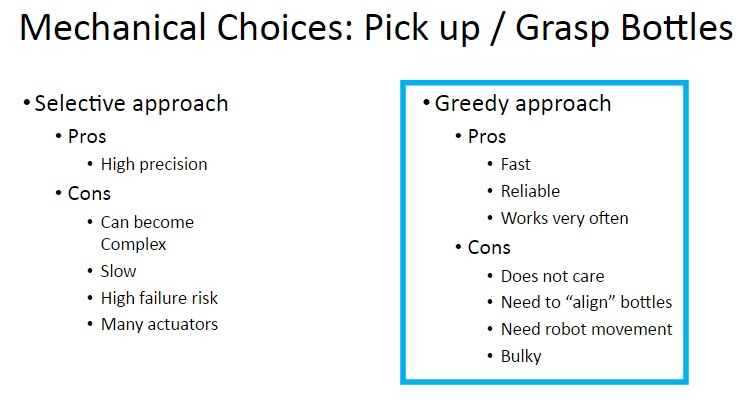
\includegraphics[width=0.9\textwidth]{PickUpApproach.jpg}
 \caption{Possible approaches for picking up a bottle.}
\label{fig:PickUpApproach}
\end{figure}

\begin{figure}[H]
 \centering
 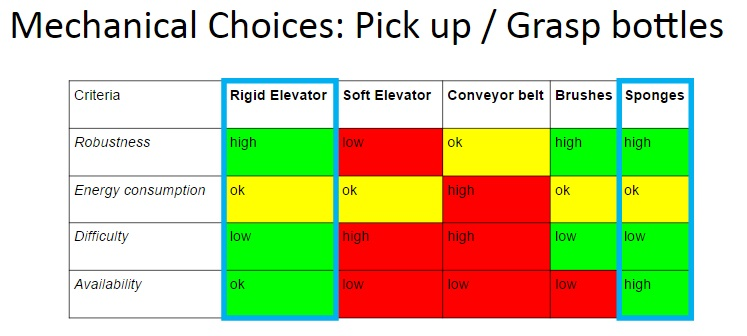
\includegraphics[width=0.9\textwidth]{PickUpChoises.jpg}
 \caption{Chart of the picking up criteria.}
\label{fig:PickUpChoices}
\end{figure}

The bottles, once collected, are placed in a storage area disposed on the robot chassis. To chose the size of the robot, we used the chart \ref{fig:TransportBottles}.

\begin{figure}[H]
 \centering
 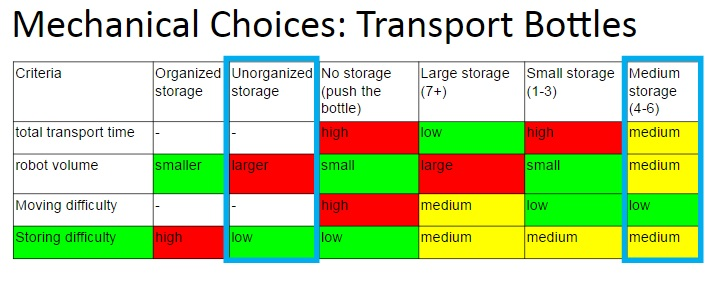
\includegraphics[width=0.8\textwidth]{TransportBottles.jpg}
 \caption{Chart of the possible solutions to transport the bottles.}
\label{fig:TransportBottles}
\end{figure}

Finally, in figure \ref{fig:ObjectDetection} is shown the chart that made us choose the sensors that allows the robot to perceive the environment and detect the bottles.                                                
\begin{figure}[H]
 \centering
 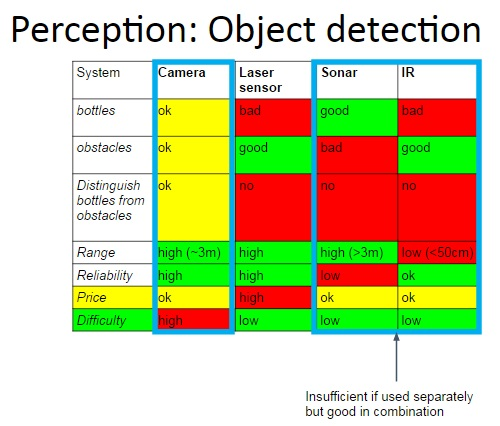
\includegraphics[width=0.7\textwidth]{ObjectDetection.jpg}
 \caption{Morphological chart for the sensors choice.}
\label{fig:ObjectDetection}
\end{figure}

\section{Division of labor}
Initially, in order to speed up the robot’s process of realization we distributed the principal tasks among the members of the team.
Three main tasks were given, one for each member of the team, in order to work in parallel, to fulfill the goal faster. These tasks were:

\begin{itemize}
\item Mechanical Part : \textit{developpment of the mechanical aspect of the robot, creation of a solidworks model, and drawings for the mechanical workshop.}
\item Electronic Part : \textit{Choice of the power, electronic components, soldering, testing and connections.}
\item Software Part : \textit{developpmemt of the algorithm, the communication protocols, image processing and scripts.}
\end{itemize}

Challenges of such an project was to respect these charts as much as possible and to stick to the plan. As it was suggested by the assistants, the evaluated time is always too short for a specific task, and the  difficult task was to determine exactly how much time a certain task or accomplishement would take. \\

Deadlines on achievements for each single part were defined according to Gantt charts that helped us to keep an overall look on the advancement of the project.
In figure \ref{fig:GanttChart1} (see Annex) is represented the first Gantt chart conceived after the decision on the main characteristics of the robot and previous to the last milestone were all the details behind our idea of the robot were to be discussed with the supervisors.\\

Another Gantt chart has been realized after the 3th milestone in order to organize the final work and it is showed in the figure \ref{fig:GanttChart2} (see Annex).\\

The division of the development of the robot in mechanical, electronic and software aspect was necessary to speed up the realization of the robot, although the lasts weeks have been dedicated to the merging of these differents parts allowing the team to work on the mechatronic of the robot and finally obtaining it with all the characteristics that had emerged during the initial brainstorming and developped during the advancement of the single parts.   
%\cleardoublepage
%\clearpage
%%%%%%%%%%%%%%%%%%%%%%%%%%%%%%%%%%%%%%%%%%%%%%%%%%%%%%%%%%%%%%%%%%%%%%%%%%%%%%%%
%
%   Semester project, fall term 2014
%   Author: Jakob Ehrl, born 01/24/91
%   Study program: Computer science, MA 1
%   
%   Professor Dr. Francesco Mondada
%   Assistant: Dr. Stefan Witwicki
%
%%%%%%%%%%%%%%%%%%%%%%%%%%%%%%%%%%%%%%%%%%%%%%%%%%%%%%%%%%%%%%%%%%%%%%%%%%%%%%%%%

\chapter{The Robot}
%(short introduction w/ pics of the robot.)
Since the beginning we aimed to develop a robot that could move in every part of the arena and theoretically capable of grasping all the bottles.
Therefore to accomplish this goal all the strategies that have been evaluated at the beginning aimed to conceive a robot whose first characteristic was robustness. All the solutions that could be specific just to a particular situation or environment have been discarded.
Keeping in mind this idea the robot’s characteristics came up as a consequence.
Indeed the first consequence was the actual size of the robot. The width had to respect the constraint to be smaller than 45 cm in order to be able to take the ramp and access to the zone 4 of the arena.
Furthermore the robot shall not have components distant from the ground less than a certain threshold, that has been decided to be of 4 cm, so that any possible contact of these components with the rocks while passing from the zone 1 to the zone 3 would be avoided.
However, in order to be able to collect bottles, the elevator couldn't respect such a constraint. Therefore when it comes to corss the rocky passage the elevator is lifted up.
Our wish was to design a small robot in order to be agile enough to easily avoid the unmodeled  obstacles represented by the bricks distributed all over the arena.
Indeed a smaller robot is more likely to avoid them with ease if compared to a bigger one that needs more precision in the maneuvers in order to accomplish the same goal.

\section{Features}
The interactions of such a system with the environment are done by exploiting sensors and actuators. 
\begin{figure}[H]
\centering
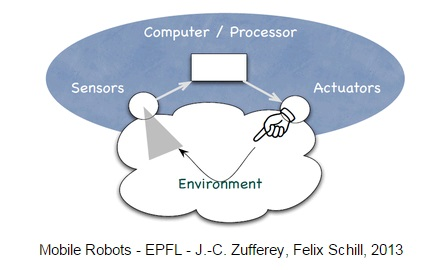
\includegraphics[width=0.8\textwidth]{RoboticSystem.jpg}
\caption{Conceptual schema of a robotic system and its interactions with the environment.}
\label{fig:RoboticSystem}
\end{figure}

As a result the main components of our robot can be clustered according to this division:
\begin{itemize}
\item Sensors
\subitem - Ultrasonic
\subitem  - IR
\subitem  - Camera
\item Brain
\subitem  - Odroid
\subitem  - Wild Thumper controller
\subitem  - 2 Arduino Micro
\item Actuators
\subitem  - 3 Servo-Actuators
\subitem  - Brush motor
\end{itemize}

Using such a system the bottles will be grasped thanks to the cooperation between the rotating brush and the mobile plate (actuated by the servo) and put in a storage area above the robot in order to stock ~4 bottles before dropping them into the recycling area opening the back door.
This storage area upon the robot was conceived since we wanted also to be able to store several bottles on the robot in order to not have to return to the recycling area each time a pet bottle was grasped.
The way of grasping bottles has been thought in way to be as much greedy as possible, meaning that detection of the exact position and orientation of the bottles had to be avoided because it would require a lot of time and precision from the sensors decreasing the robustness of the solution since in case of unforeseen difficulties it would get stuck in a dead end.
Therefore the way to pick up bottles resulted in a mobile plate that aided by a moving brush sponge could retain the bottles until the  plate reach a position from where the bottles can roll in the storage part upon the robot.
The moving plate is shaped in a way that bottles don’t need to be perfectly aligned  to be grasped by the “pick-up bottle” system. Furthermore the brush can slightly move in a range of $\pm 5^{\circ}$ Avoiding the possibility of a bottle getting blocked under it.
 This characteristic has been exploited also to detect when a bottle was actually grasped. Indeed getting in the contact with a bottle, the brush had to generate more force to displace it. This change could be felt by the motor of the sponge in terms of a change in the current that could be read by the “brain of the robot”

\section{Mechanical principle}

\begin{wrapfigure}{l}{0.5\textwidth}
\begin{center}
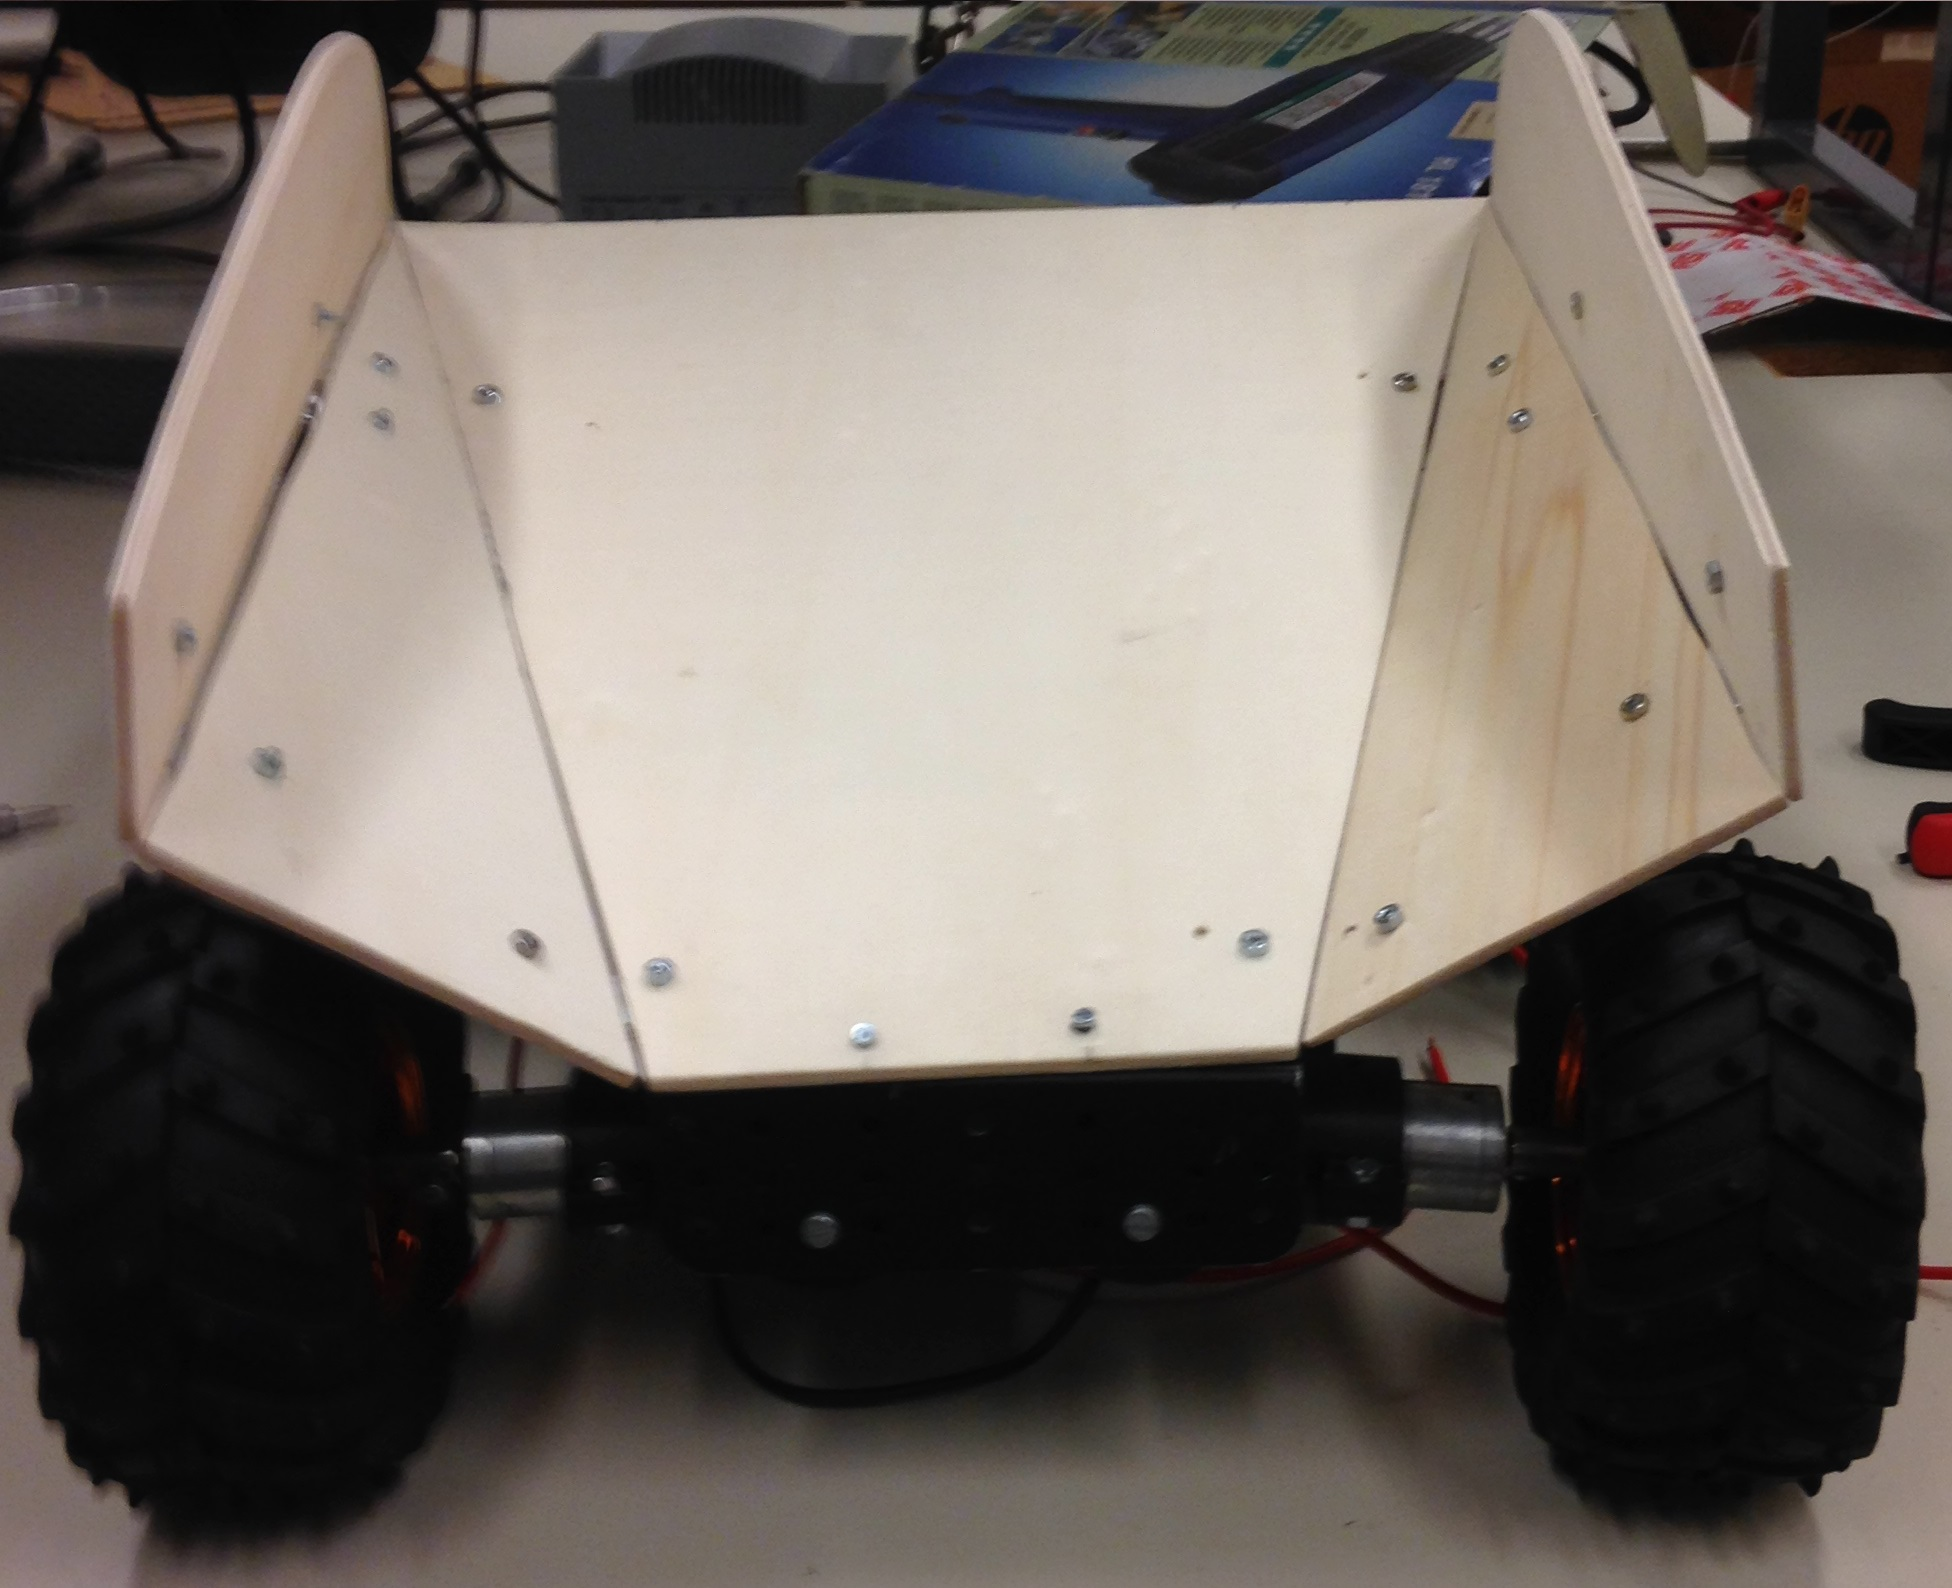
\includegraphics[width=0.3\textwidth]{WoodenModel1.JPG}
\end{center}
\caption{Back view of the robot's wooden model.}
\label{fig:WoodenModel1}
\end{wrapfigure}

After deciding the robot’s working principles, in order to verify the effectiveness of our ideas, some tests of the single components constituting the robot have been conducted.
Firstly, a wooden model of the principal parts has been realized.
%Some pics of this model from different points of view are %shown in the figures below. 


During this process the experiment conducted on it allowed us to realize some small changes that have made our initial draft evolve toward the final idea.

These tests were useful to determine the effectiveness of the “pick-up bottle” system and to comprehend in which cases the bottles could get stuck in undesired positions. This made us modify the shape of the elevator removing the lateral walls that represented an obstacle for bottles not perfectly centered with respect to the center of the robot.


\begin{wrapfigure}{r}{0.5\textwidth}
\begin{center}
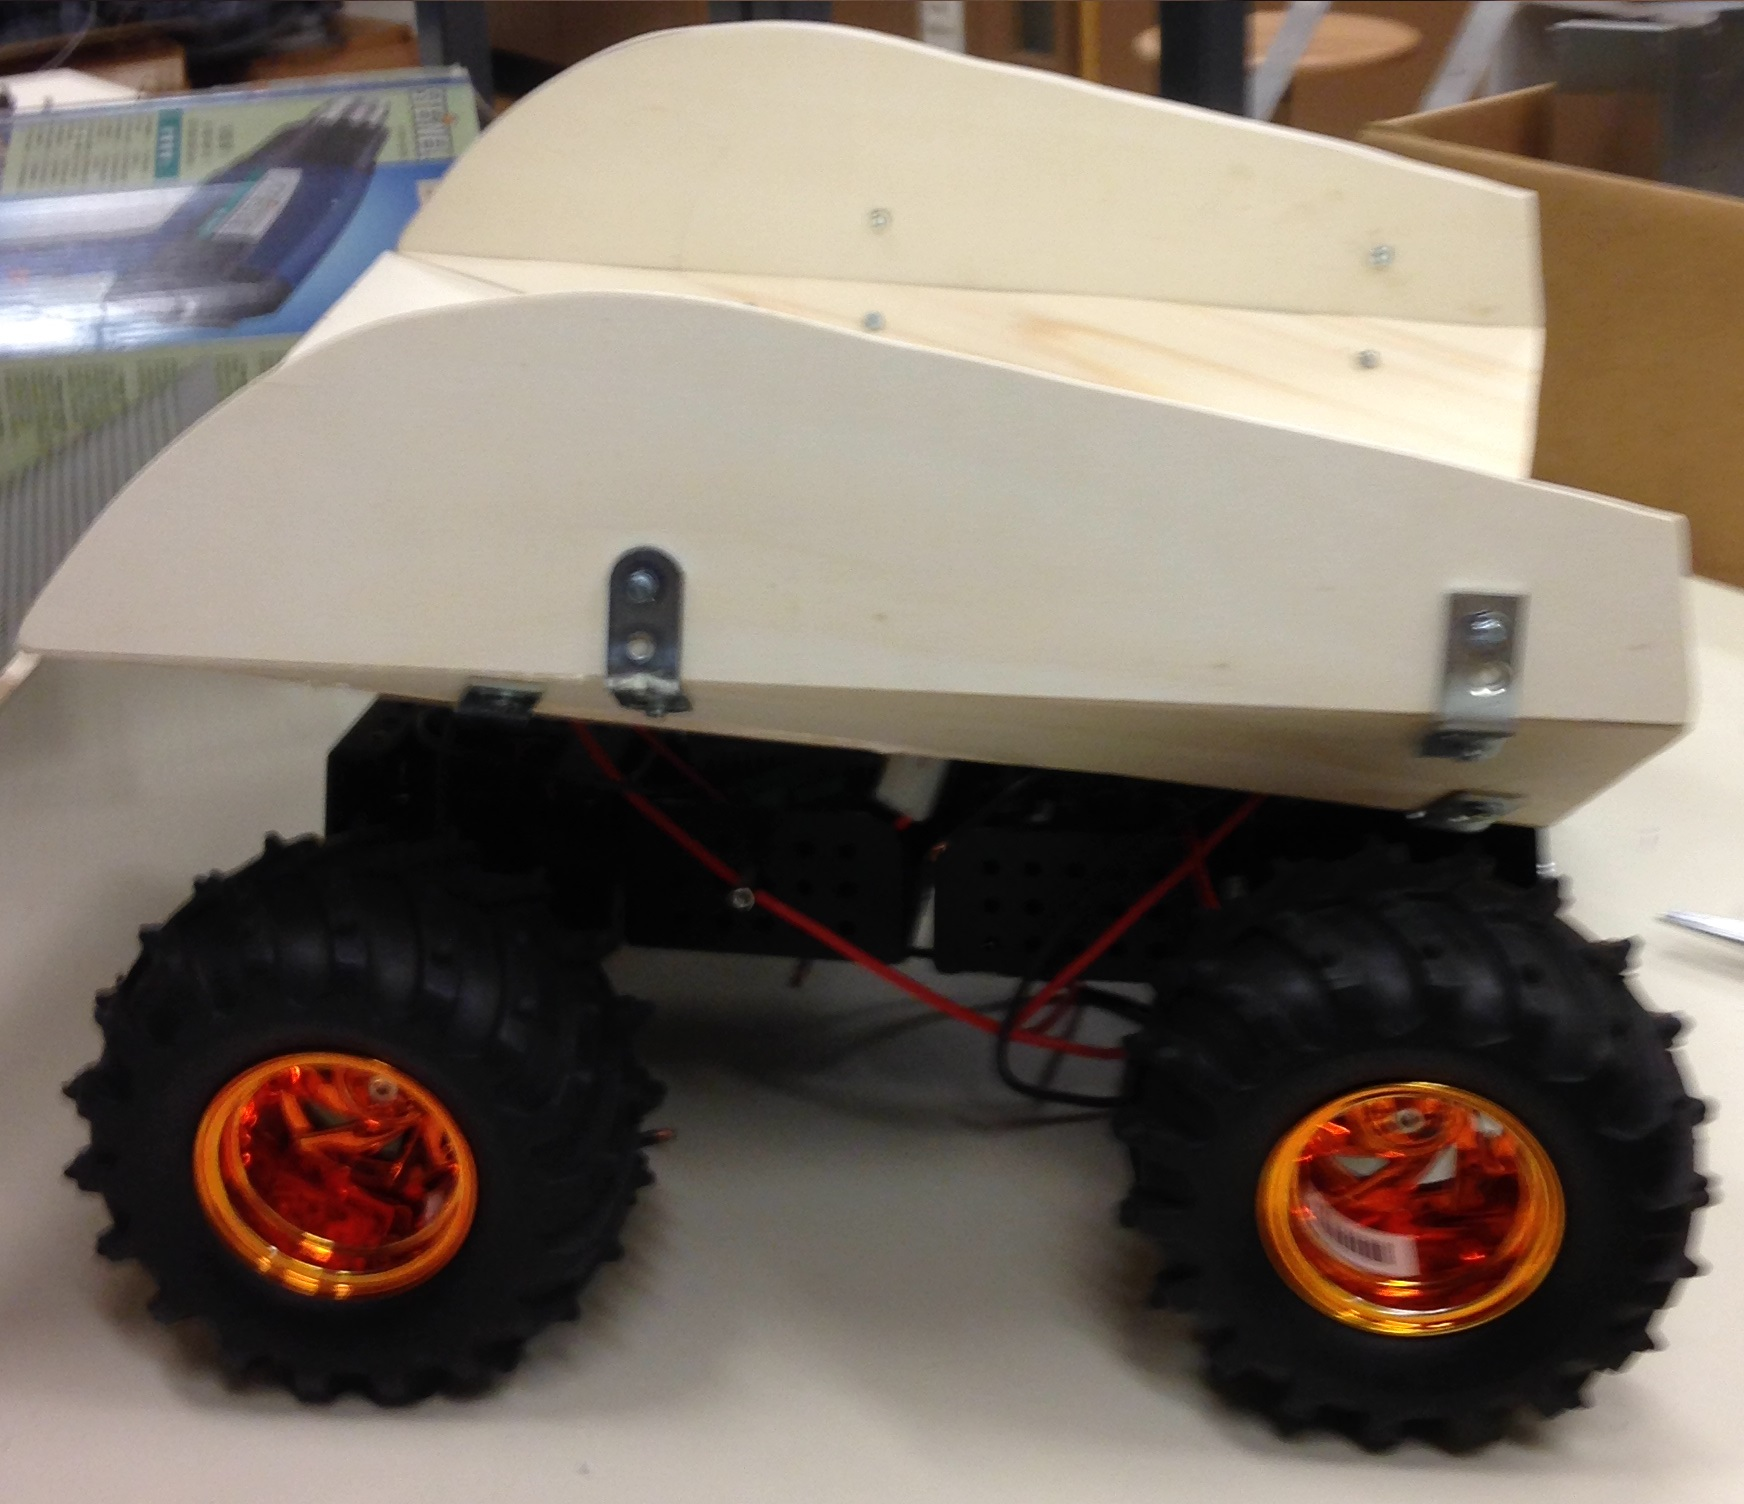
\includegraphics[width=0.3\textwidth]{WoodenModel2.JPG}
\end{center}
\caption{Lateral view of the robot's wooden model.}
\label{fig:WoodenModel2}
\end{wrapfigure}

Furthermore we shaped it in a more rounded fashion in order to allow even almost bottles vertically oriented to be successfully collected by the robotic system by turning within the elevator thanks to the help of the curvature.

These modifications pointed toward the obtainment of a “greedy” mechanism that could deal with almost every possible situation, even the most challenging ones.
Furthermore, the tests on the wooden model, have made possible the optimization of the storage part in terms of:

\begin{itemize}
\item Number of bottles that could be stored
\item Space for electronics
\end{itemize}

\begin{wrapfigure}{l}{0.5\textwidth}
\begin{center}
 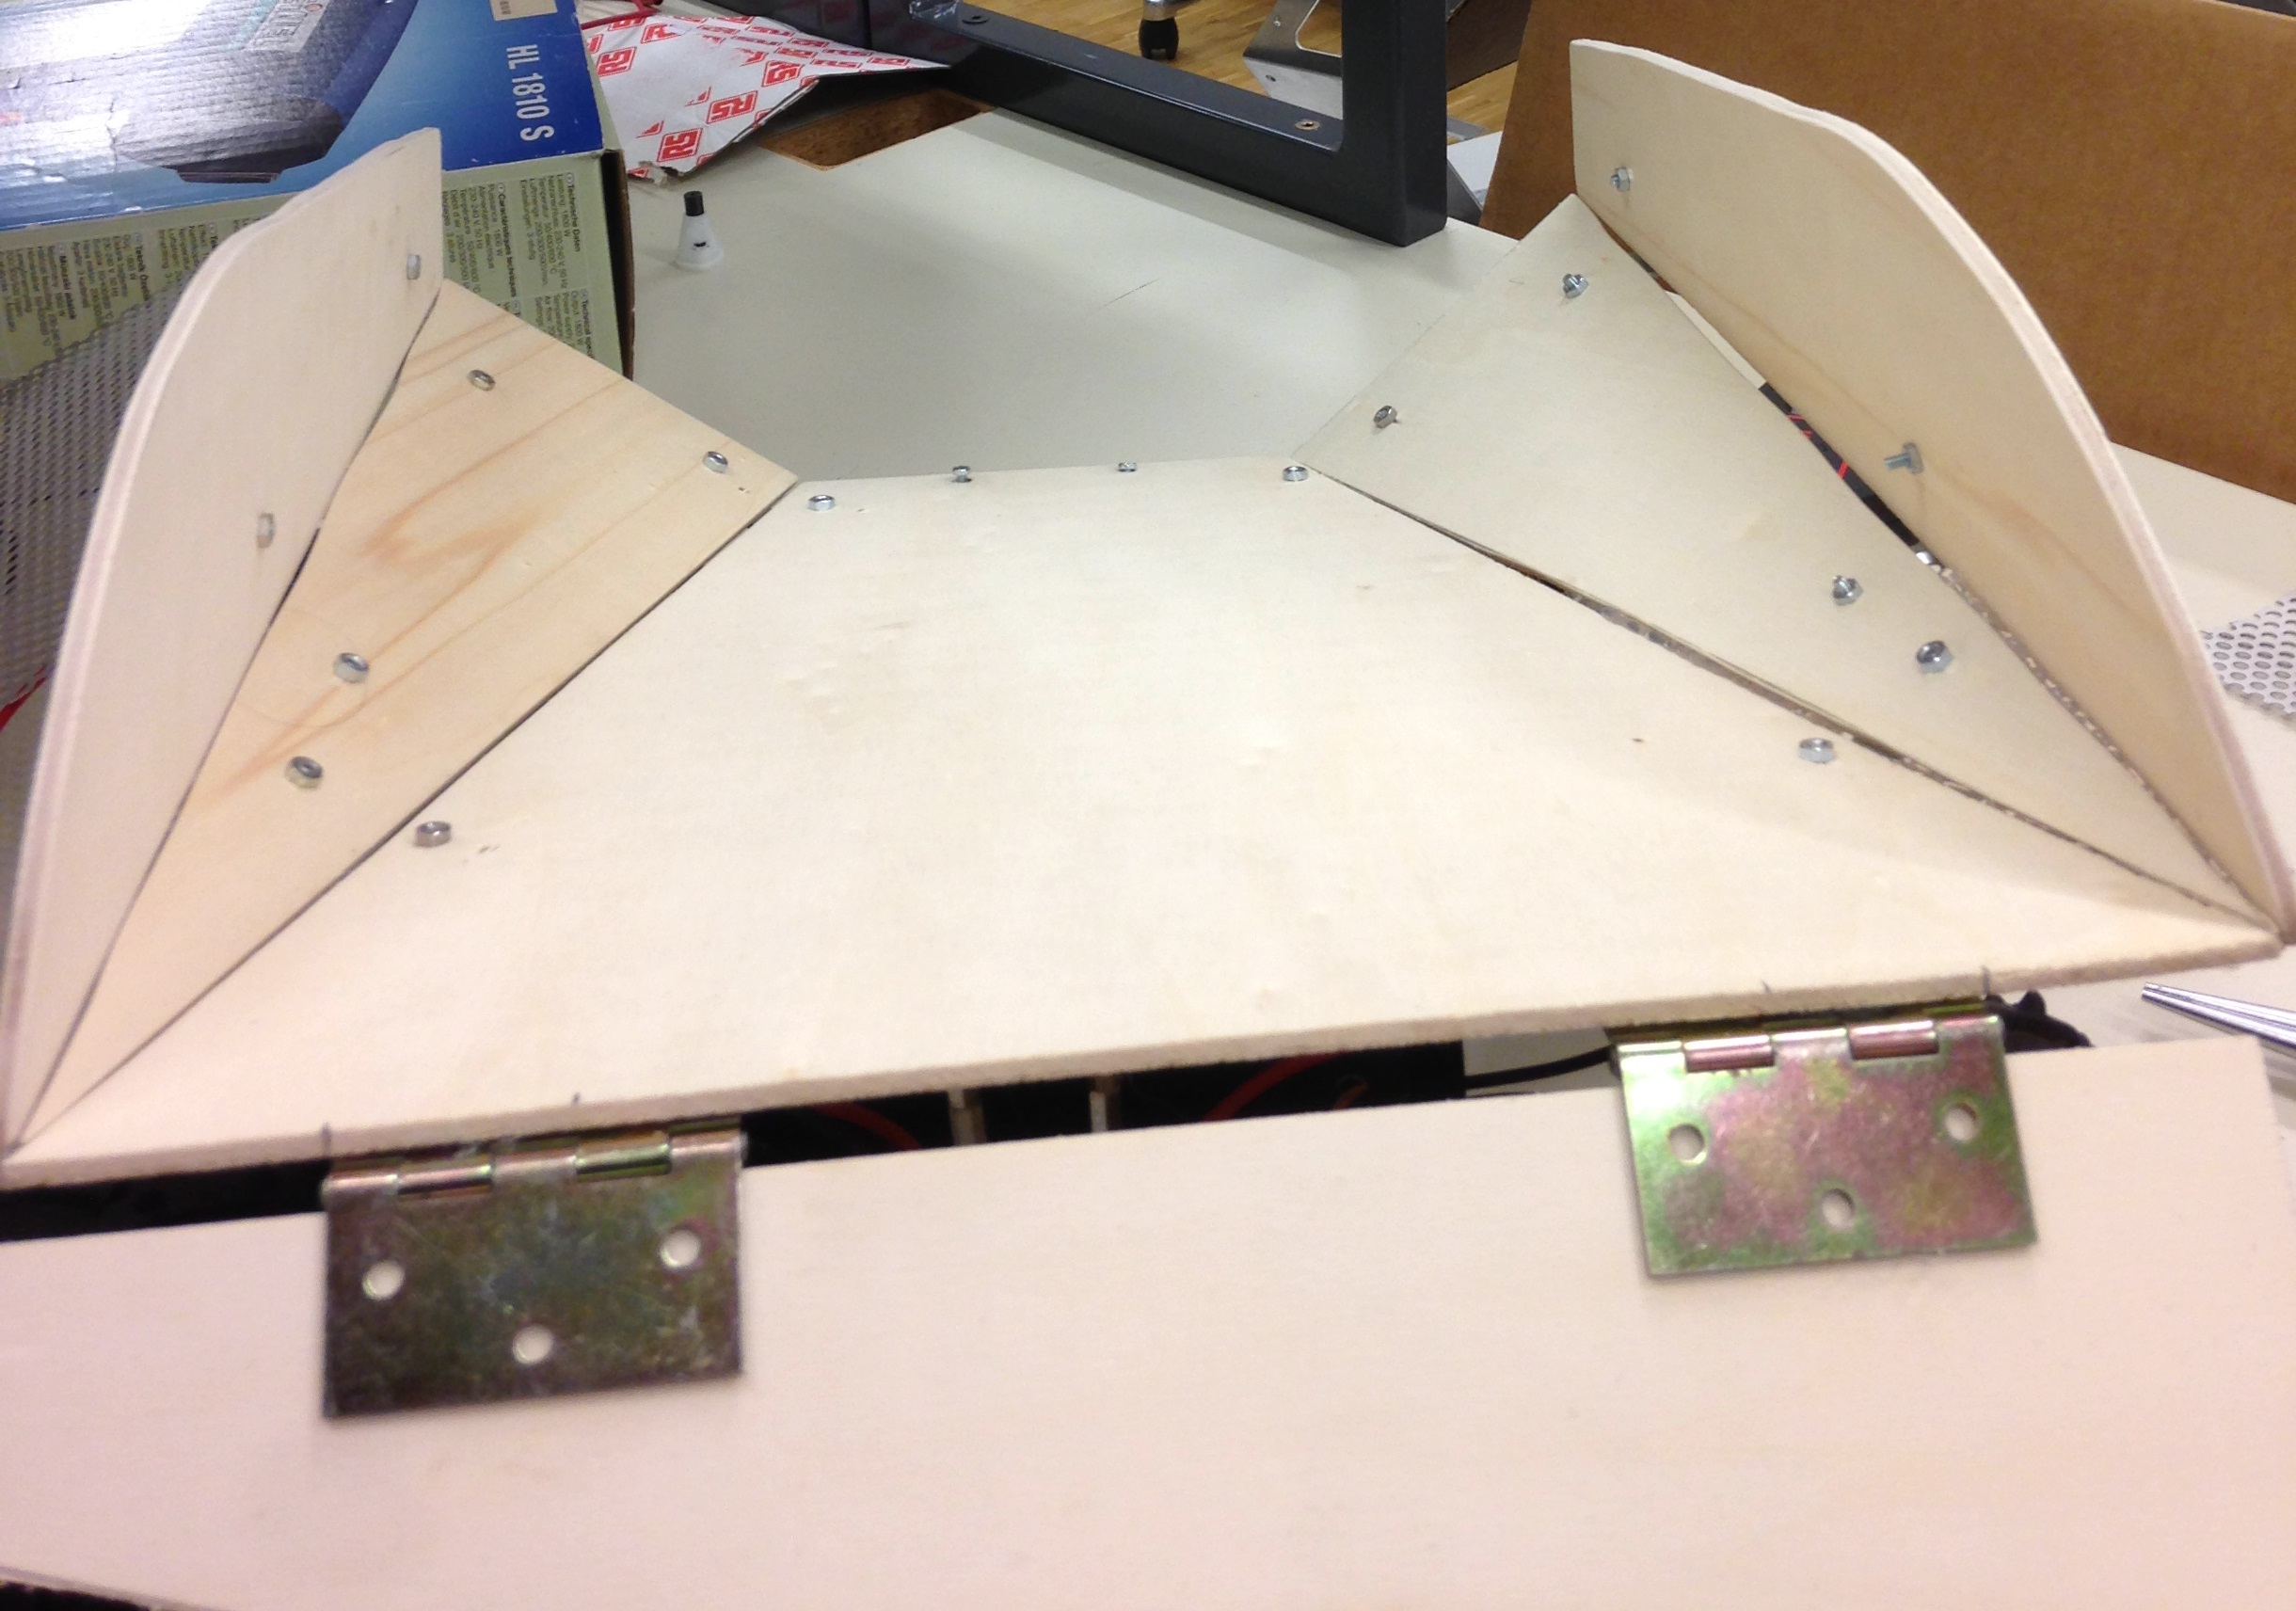
\includegraphics[width=0.3\textwidth]{WoodenModel3.JPG}
\end{center} 
 \caption{Upper-Front view of the robot's wooden model.}
\label{fig:WoodenModel3}
\end{wrapfigure}

Indeed below the storage plate there is an hidden space that was decided to be reserved for the electronic components in order to guarantee a compact design where no space is wasted as wanted since  the beginning.
Thus all the electronics has been disposed under the storage part of the robot that is attached to the robot in a way to form a ramp in order to favorize the rolling of the bottles coming from the moving plate.
Moreover, this ramp was conceived in a way that its height is adjustable, simplifying a lot the assembly of the final robot without incurring in unpredicted inaccuracies.
This adjustable slope mechanism is depicted by the Figure \ref{fig:AdjustableHeight3} below.

\begin{figure}[H]
 \centering
 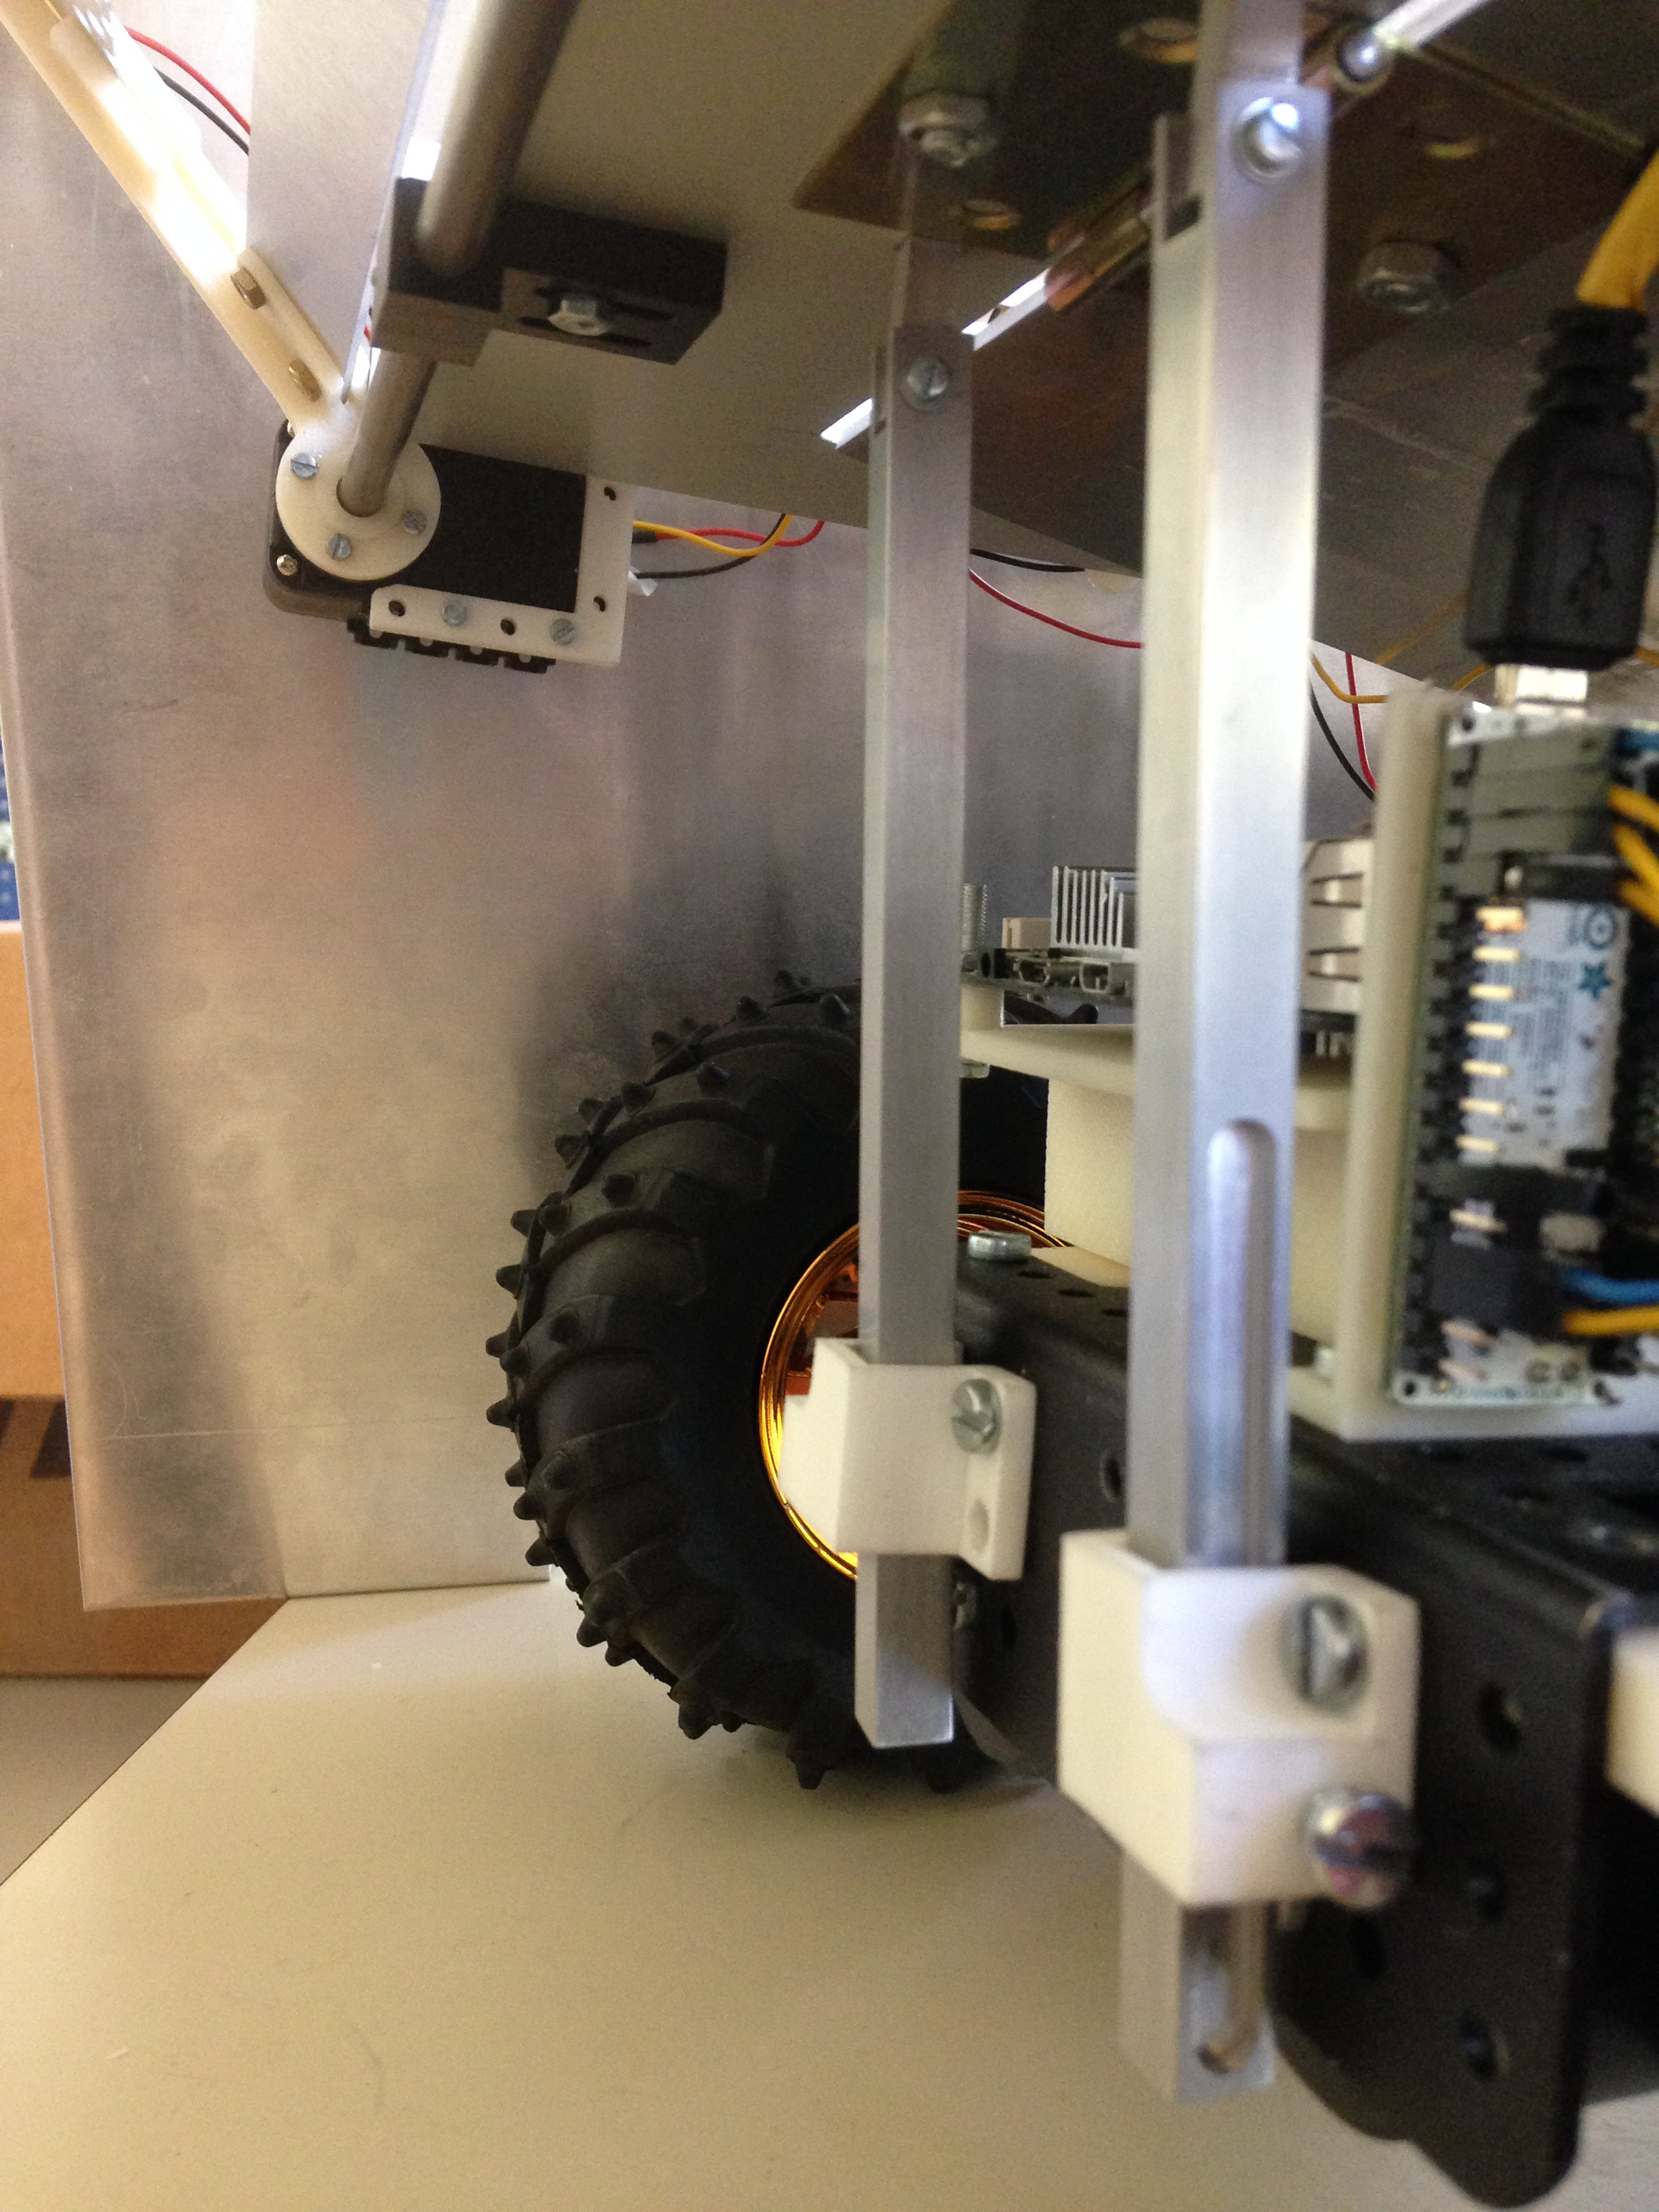
\includegraphics[width=0.5\textwidth]{AdjustableHeight3.JPG}
 \caption{Adjustable height mechanism of the storage compartement.}
\label{fig:AdjustableHeight3}
\end{figure}

After some test the slope for an aluminum plate that allowed the bottles to roll without getting stuck resulted to be of about 30°.
Furthermore, the electronics has been arranged in a way to allow an easy access to it and in particular for what it concerns the disposition of the batteries.

Thanks to the good quality of the described model manufactured in wood we have even been able to test on it the real actuators that afterwards has been used on the final model.
Being satisfied with this first mechanical verification of our idea a SolidWork model of the final robot has been realized.
This model is represented in figure z.

(((((((((((((((((((((((((((((((((FIGURE)))))))))))))))))))))))))))))))))







After the approval of all the team members about the mechanical components that would have constituted the final robot, the mechanical 2D plans of all the single components have been produced to be then sent to the mechanical workshop and be manufactured.
More complex parts have been printed with the further benefit of saving time having the available to be tested far earlier than the aluminum parts.
 In the meantime the “holders” of the sensors have been printed together with the electronic parts’ boxes that have been conceived in order to guarantee their arrangement in the reserved space in the most proper way and allowing at the same time an easy access to them.
In the mechanical conception of the robot, great importance has been given to the design of the elevator shown in Figure a.

(((((((((((((((((((((((((((((((((FIGURE)))))))))))))))))))))))))))))))))


A lot of effort has been expended in order to make the electronic area, and in particular the zone reserved to batteries, easily accessible.
The storage compartment, indeed, can be detached in correspondence of the “adjustable height mechanism” and rotate around a pivoting system placed in correspondence of the end of the chassis.
The pivoting system just described is shown in Figure x

\begin{figure}[H]
 \centering
 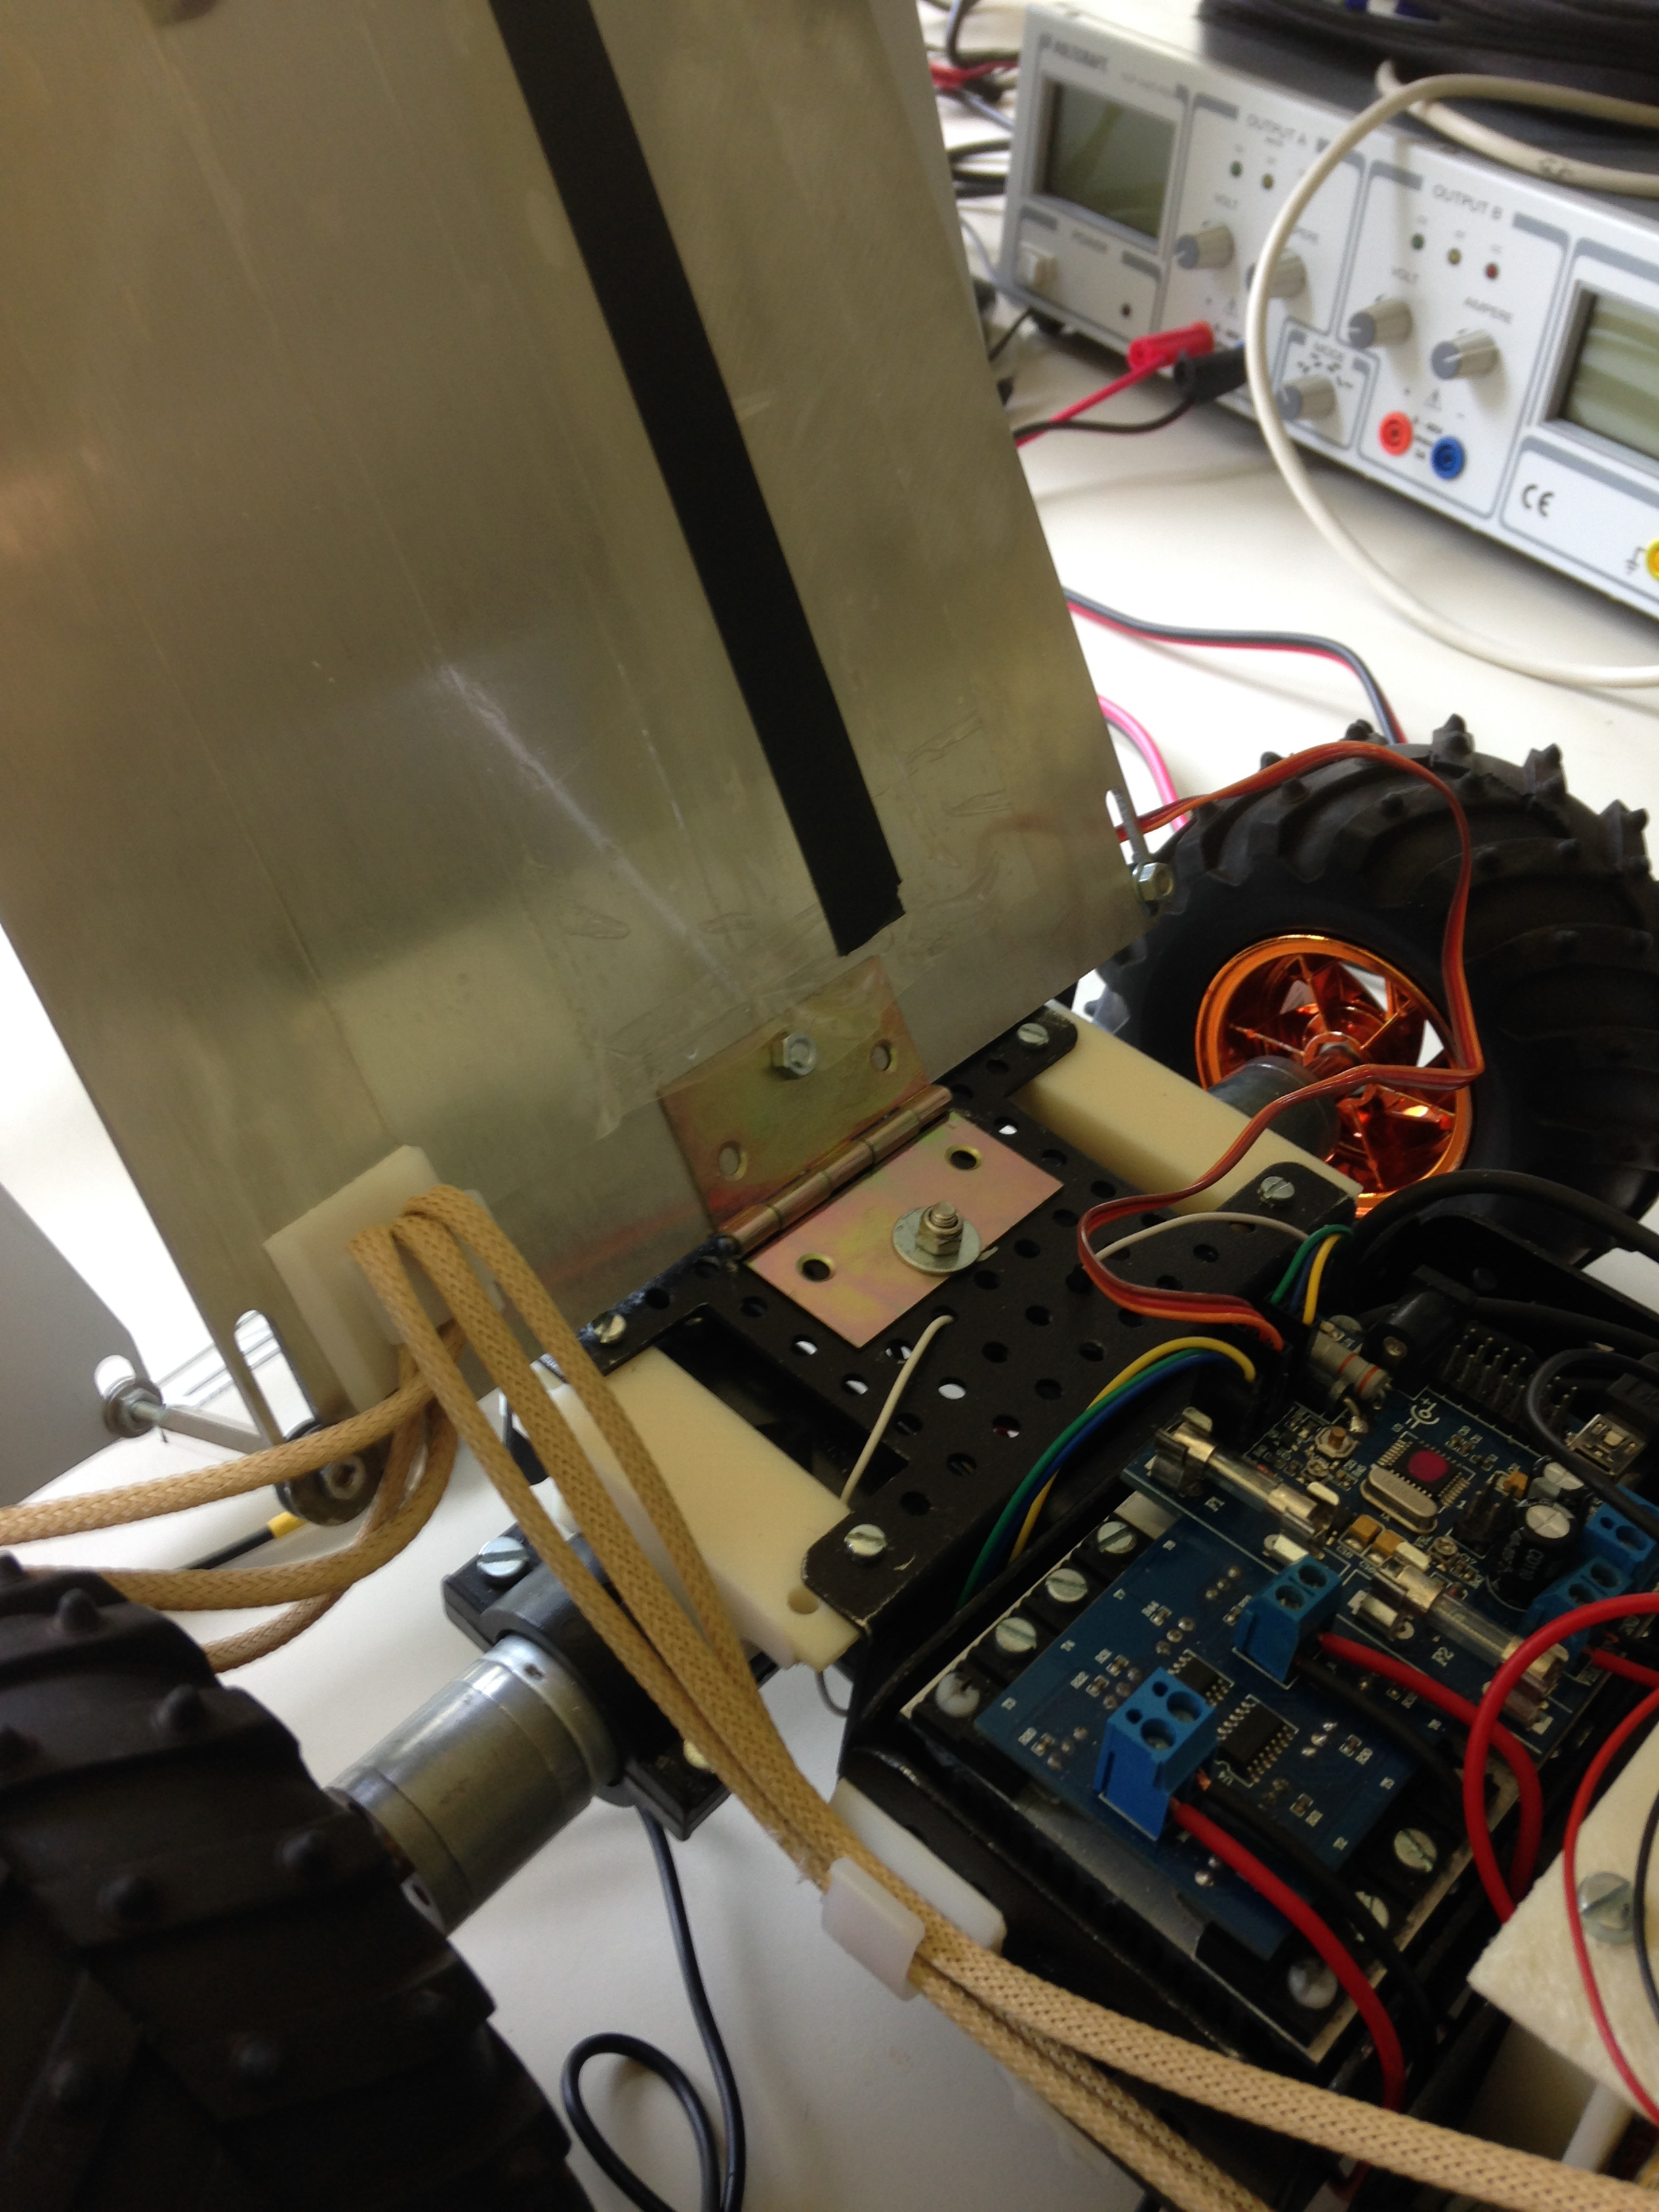
\includegraphics[width=0.5\textwidth]{PivotingSystem.JPG}
 \caption{Pivoting system for the storage ramp opening.}
\label{fig:PivotingSystem}
\end{figure}

This simple mechanism allows, as already said, to access to the electronics that’s arranged with the help of boxes which, as it can be seen in Figure y, make it possible to add and remove the batteries without having to remove any other component.

(((((((((((((((((((((((((((((((((FIGURE)))))))))))))))))))))))))))))))))

Another important feature, in terms of the mechanical conception of the robot, is the possibility to regulate the pointing direction of some sensors.
Indeed, as it can be seen in Figure 1 and Figure 2, both the camera and the two front ultrasonic sensors are holded by means of holders that allow to change the pointing direction

\begin{figure}[H]
 \centering
 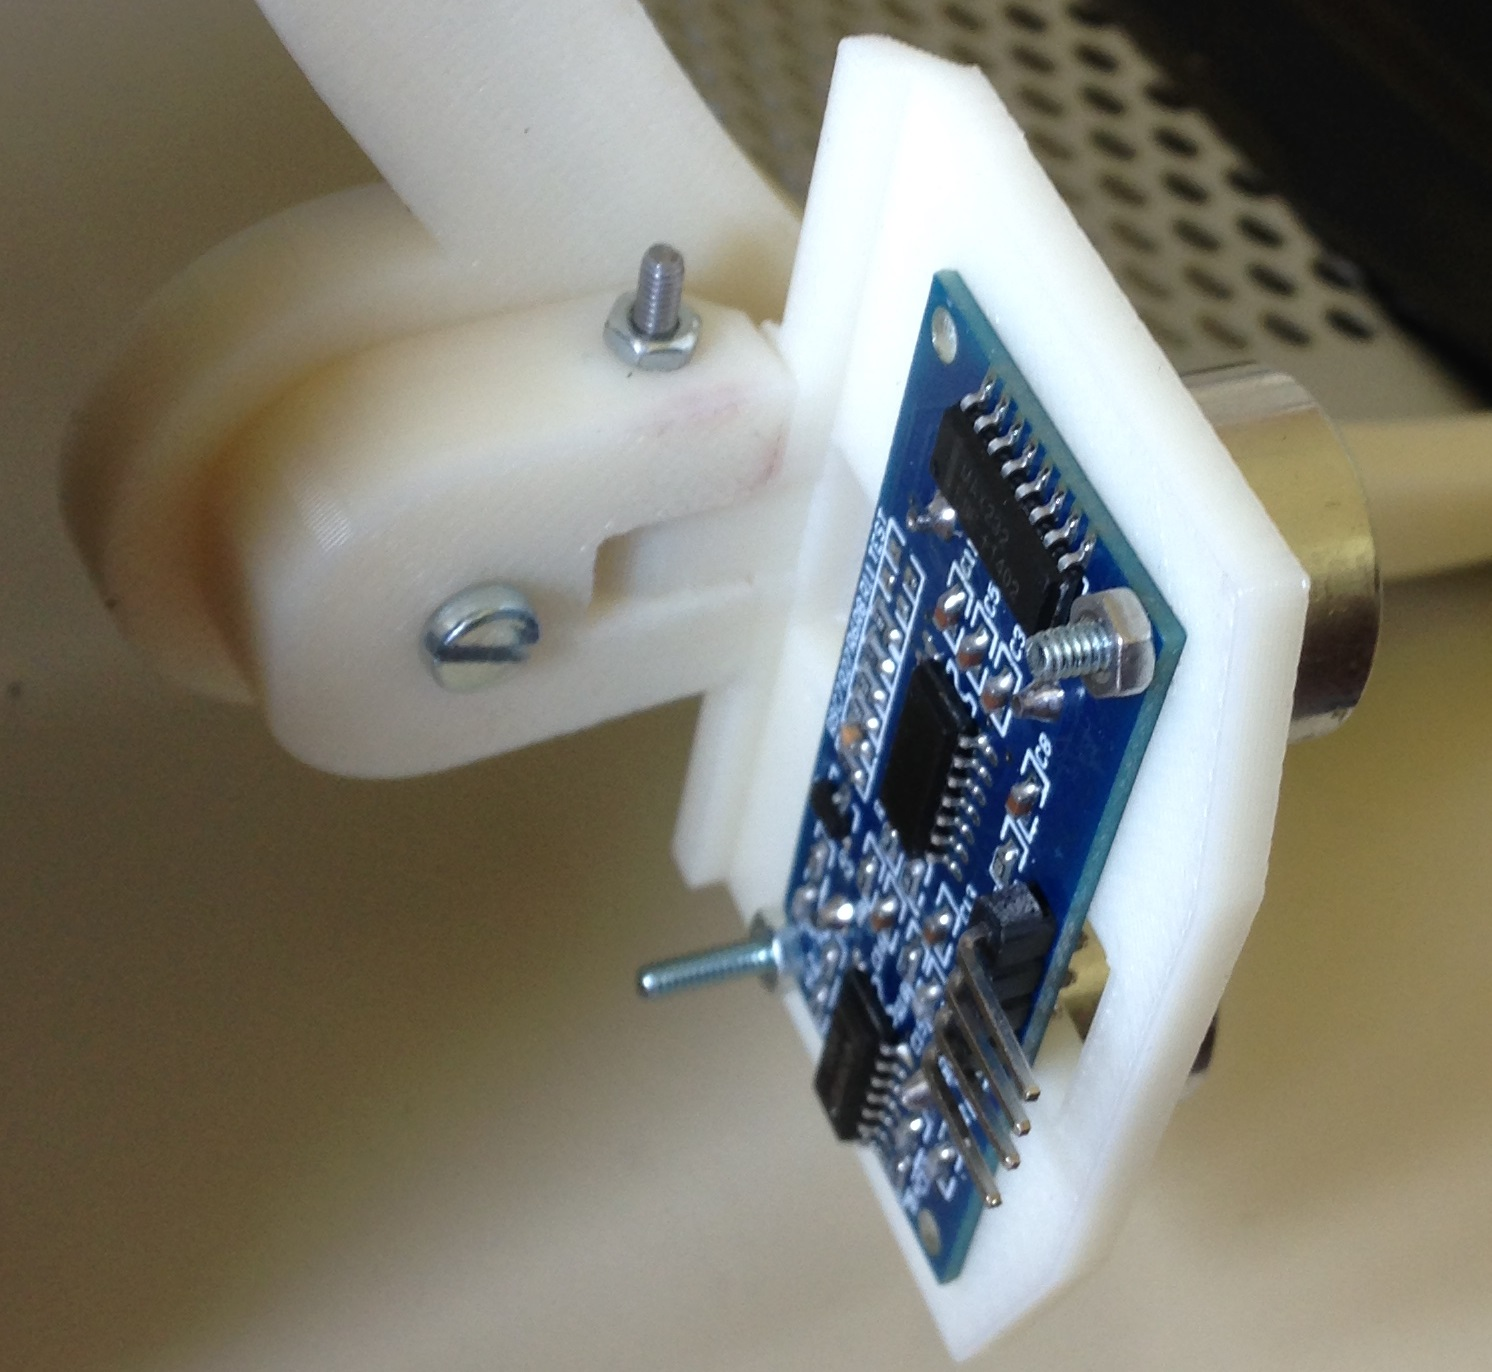
\includegraphics[width=0.4\textwidth]{PointingUS.JPG}
 \caption{Close view of the system that allows to regulate the Ultrasonic sensors' direction.}
\label{fig:PointingUS}
\end{figure}

\begin{figure}[H]
 \centering
 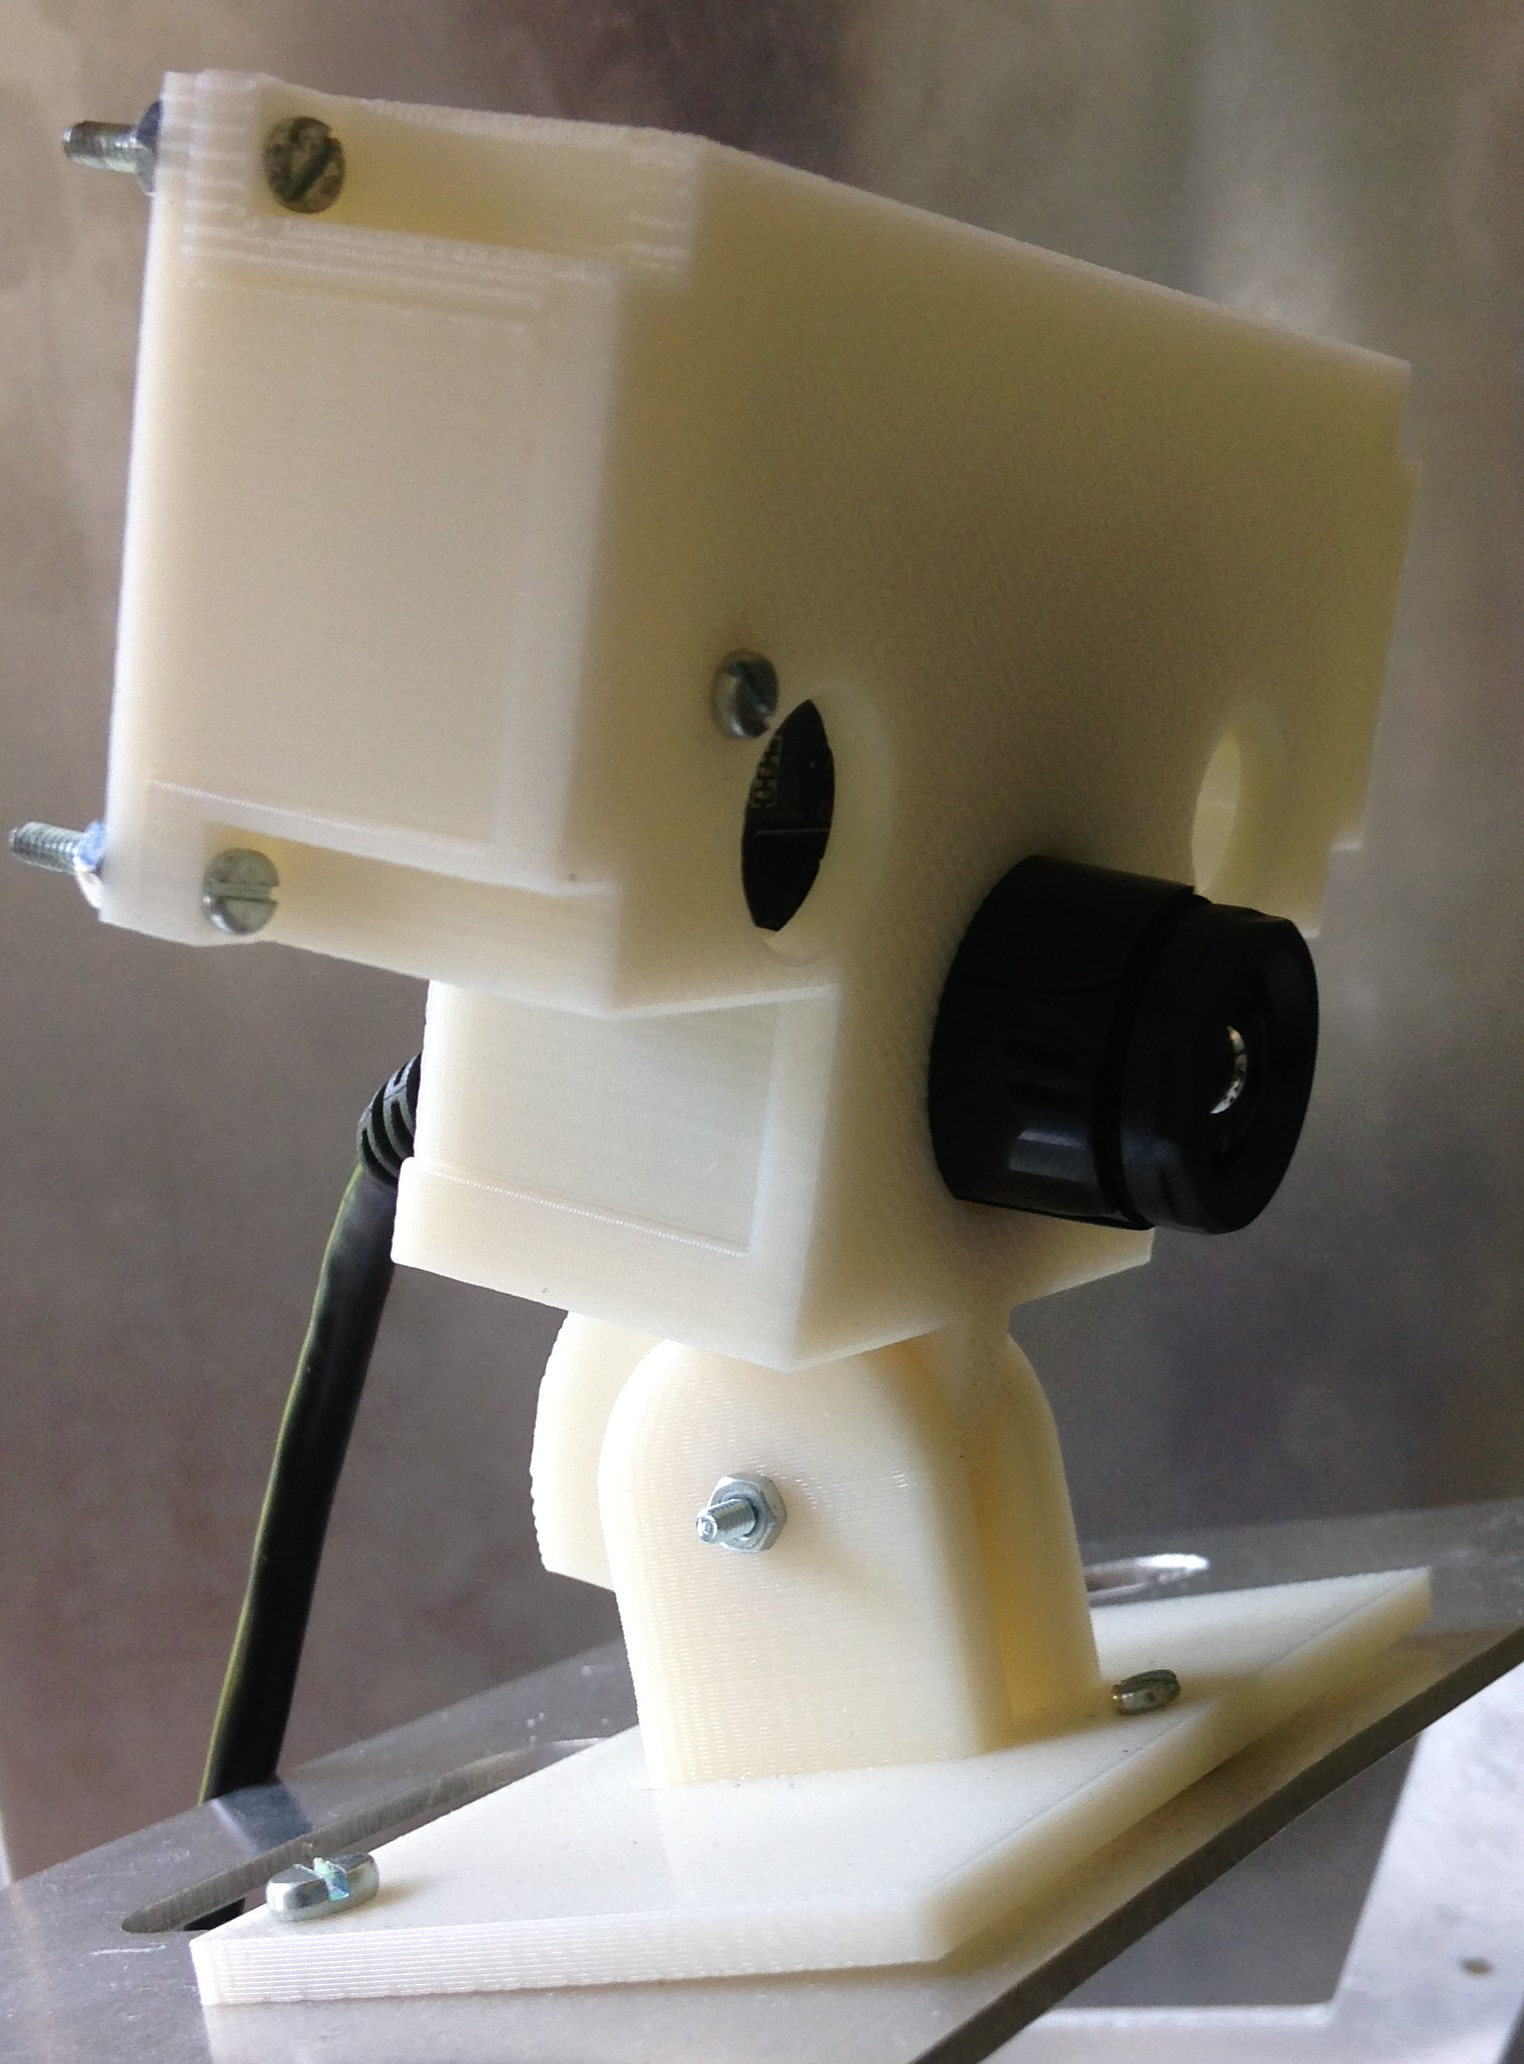
\includegraphics[width=0.4\textwidth]{PointingCamera.JPG}
 \caption{Close view of the system that allows to regulate the camera direction.}
\label{fig:PointingCamera}
\end{figure}

This was done since it was difficult to define “a priori” the arrangement that would return the best feedback in term of detection.
\section{Modules presentation}
All the robot's main functions: actuations, processing and sensing, were performed by different modules. The reason for this separation was to have microcontrollers dedicated for one purpose, thus optimizing the calculation time and efficiency of the robot. In our robot, Four main modules were working together, and each of them had specific roles...   % (\chapter{})
%\cleardoublepage
%%%%%%%%%%%%%%%%%%%%%%%%%%%%%%%%%%%%%%%%%%%%%%%%%%%%%%%%%%%%%%%%%%%%%%%%%%%%%%%%
%
%   Semester project, fall term 2014
%   Author: Jakob Ehrl, born 01/24/91
%   Study program: Computer science, MA 1
%   
%   Professor Dr. Francesco Mondada
%   Assistant: Dr. Stefan Witwicki
%
%%%%%%%%%%%%%%%%%%%%%%%%%%%%%%%%%%%%%%%%%%%%%%%%%%%%%%%%%%%%%%%%%%%%%%%%%%%%%%%%%

\chapter{Modules}

All the robot's main functions: actuations, processing and sensing, were performed by different modules. The reason for this separation was to have microcontrollers dedicated for one purpose, thus optimizing the calculation time and efficiency of the robot. In our robot, Four main modules were working together, and each of them had specific roles.

\section{Sensors Module}
The sensors Module is an arduino micro that is connected to the following
\begin{itemize}
\item 5 Infrared sensors, for obstacle detection.
\item 4 Ultrasound sensors, for bottle detection.
\item One DC brush motor driver, for the control of the frontal brush.
\end{itemize}

The task of the Arduino is to constantly receive data from the ranging devices, as well as the current measurements from the DC motor driver, transmit its data to the central processing module, and if commanded to do so, control the driver which is connected to the frontal brush motor. 

\subsection{Sensor Choices and Strategy}
During the first weeks of the semester, different sensors were purchased, and tests were performed on them, in order to have a better choice for the selection of the sensors that would be used on the robot. 


\subsubsection{The Infrared Sensor}
The Infrared sensor that was available from the virtual marked was a GP2Y0A21YK, a sensor from Sharp. 

\begin{figure}[H]
  \centering
  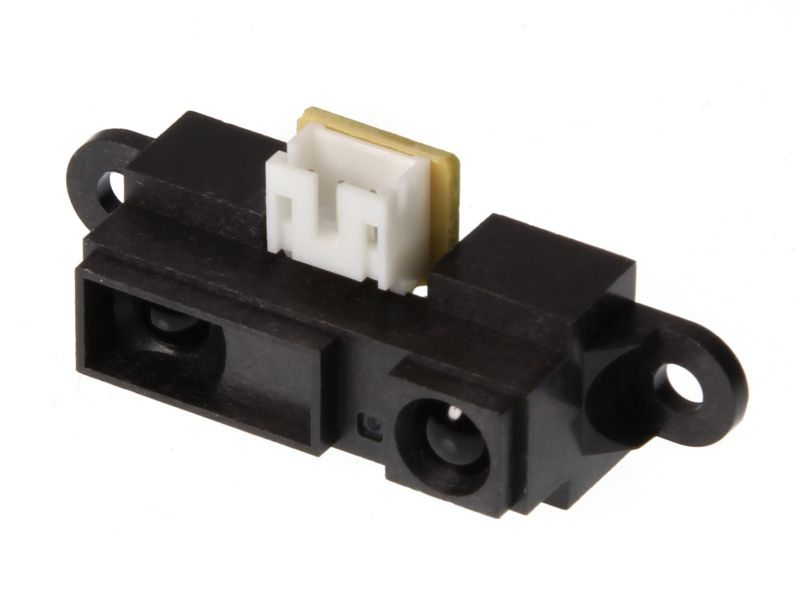
\includegraphics[width=0.3\textwidth]{IR.jpg}
  \caption{GP2Y0A21 Infrared sensor.}
\label{fig:IR}
\end{figure}

The sensor had a range up to 80 cm, which was quite far, however it had some problems detecting transparent bottles, as the IR wave would go through the bottle. Therefore, the sensor was used in detecting obstacles and solid opaque objects, as a collision avoidance strategy. In the robot, 5 of those sensors were used, two in the front, one on each side, and one on the rear, for controlling collisions while going backwards.

For measuring the distance effectively, as the relation between the voltage output of the sensor and the distance was not linear, a linear regression method was used with the measured values in the datasheet of the sensor.

\subsubsection{The Ultrasonic Sensor}

The HC-SR04 is a ultrasonic sensor, that functions with two signals: Echo and Trig. For simplicity, it was tested to combine these two lines into one, with a resistance in between, and changing the state of the pin on the arduino everytime we would measure the signal. However, tests proved that the sensor worked less well than with two pins in this configuration, so two pins were used instead. The range was up to 4 meters, however, as this range was useless, the range was decreased to 1.3 meters. The decrease in range also allowed the signal to be faster, since the arduino is waiting for a pulse input when reading the sensor value, and at closer range the pulse comes back faster. A timeout was used to enforce the range limitations. 

\begin{figure}[H]
  \centering
  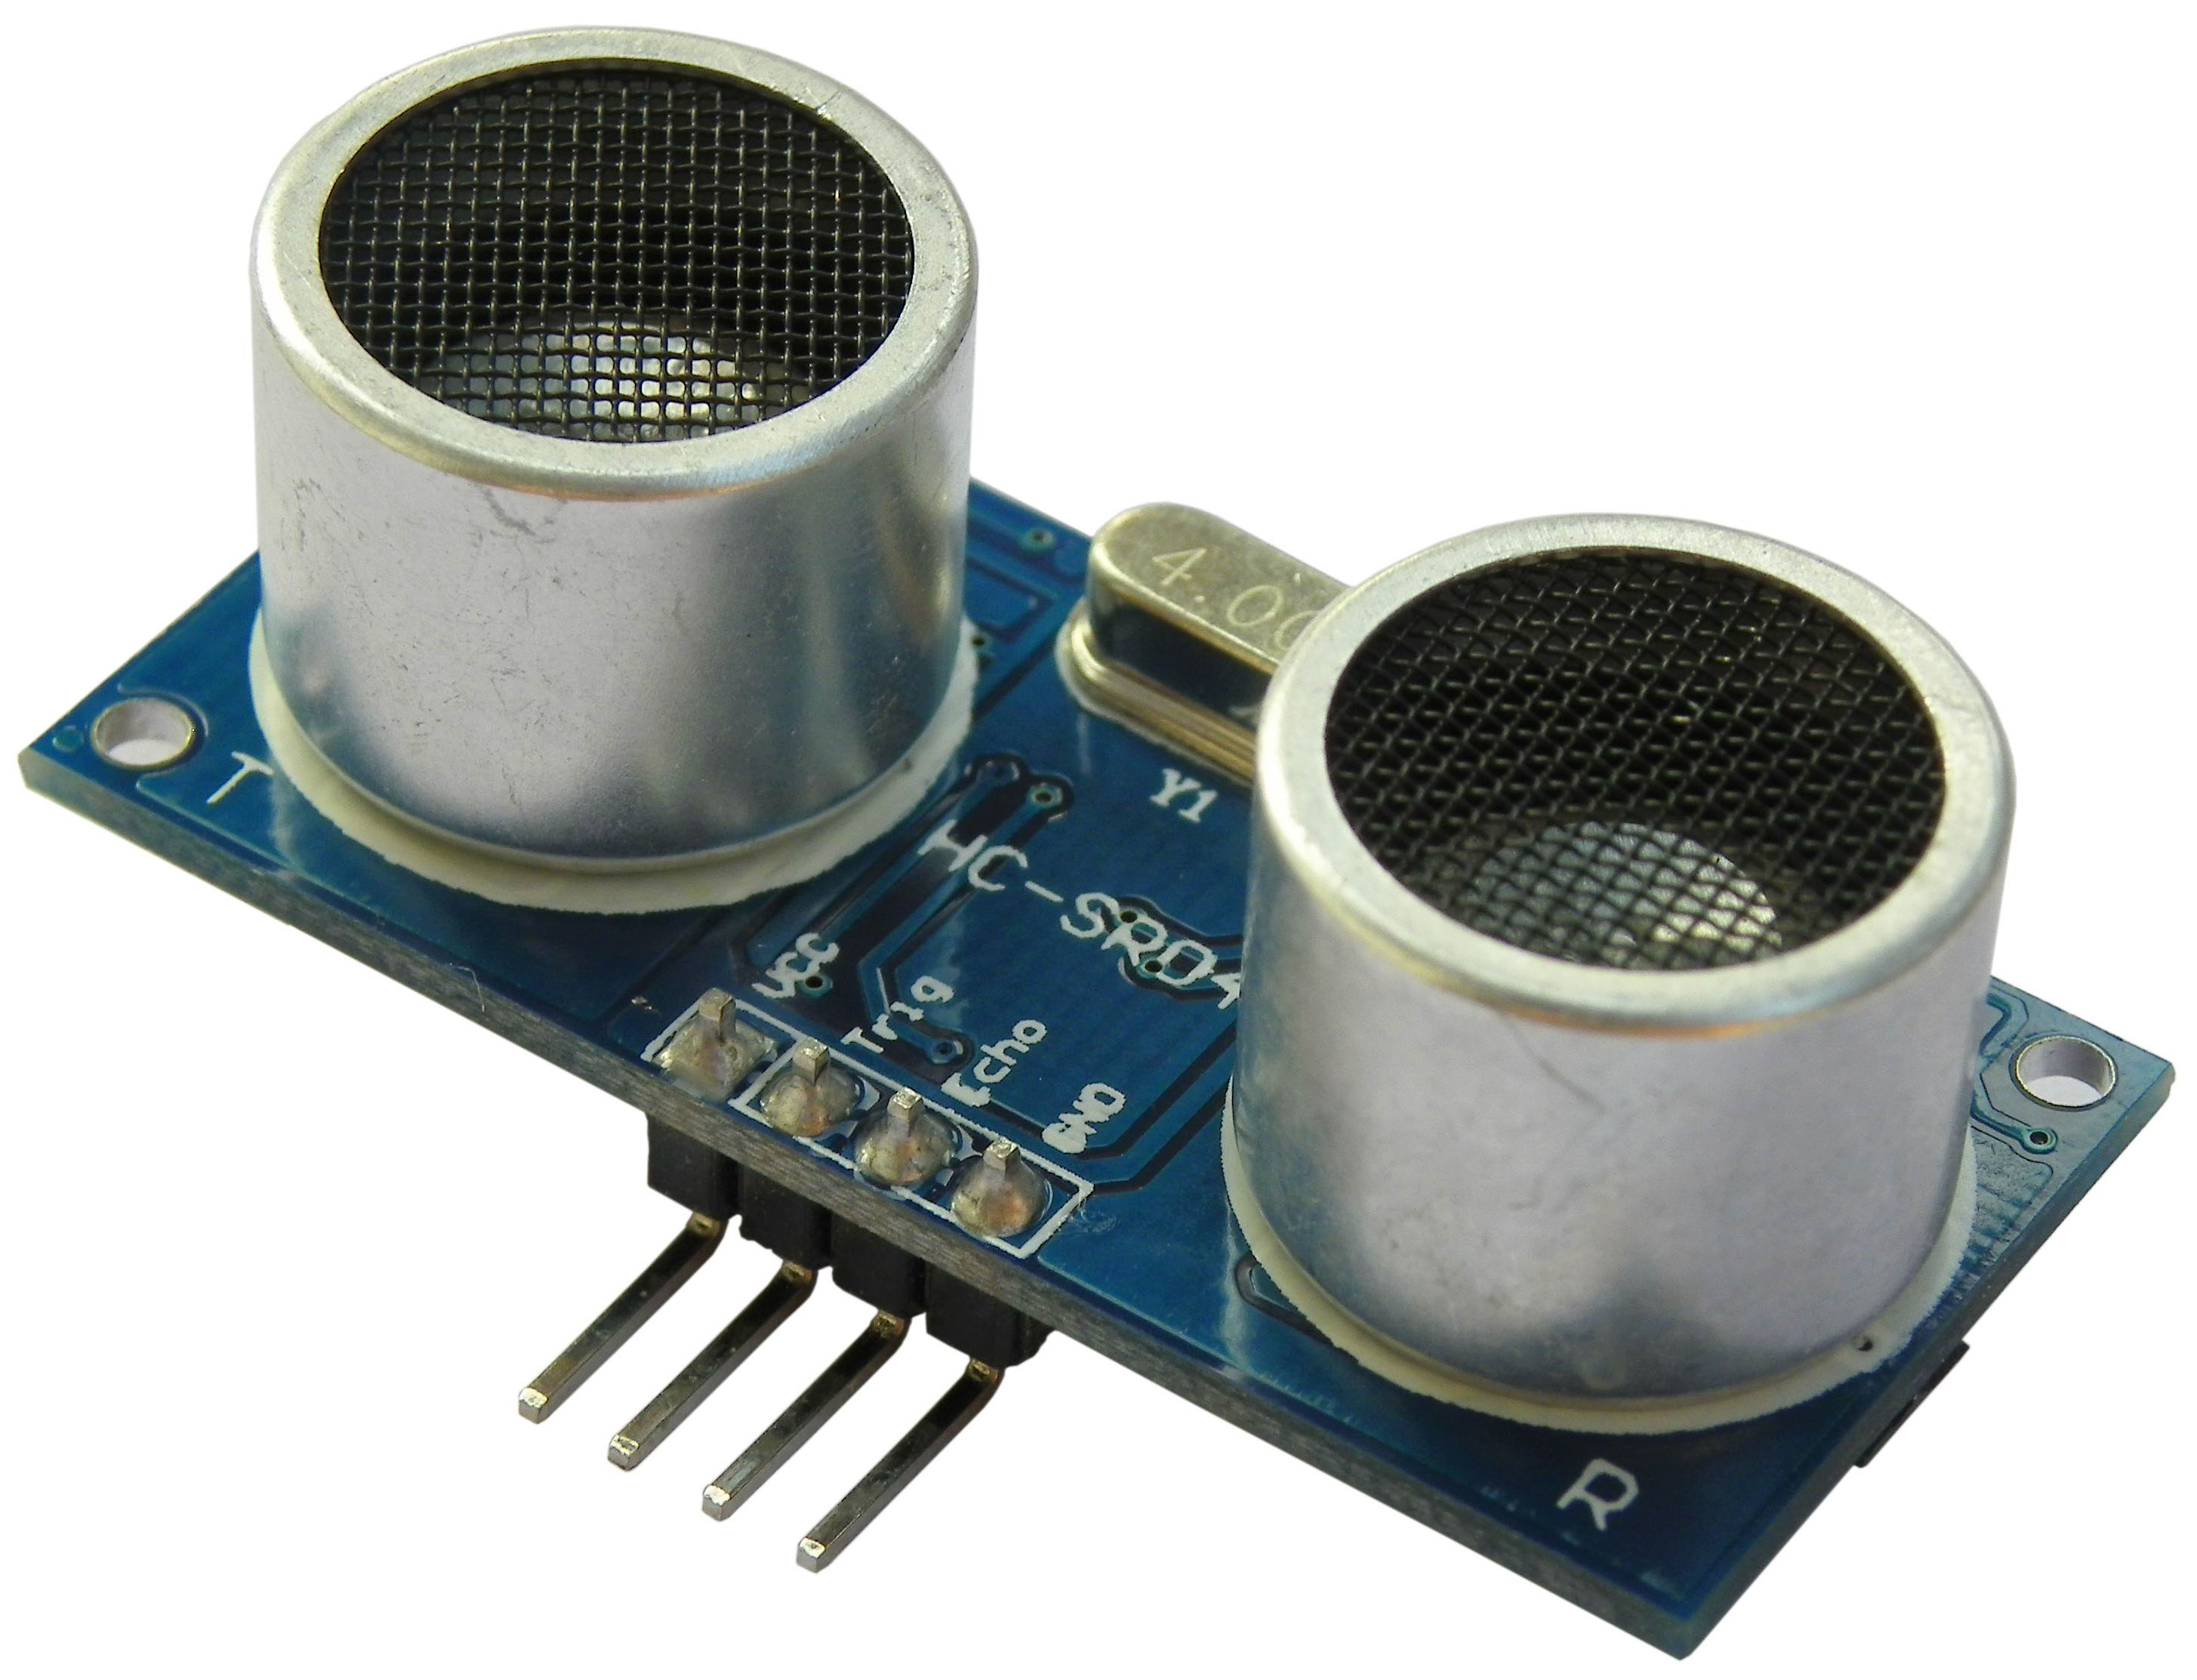
\includegraphics[width=0.3\textwidth]{US.jpg}
  \caption{HC-SR0 Ultrasonic sensor.}
\label{fig:US}
\end{figure}

All in all, the sensor worked quite well with complex shaped objects, but on a flat surface that is not perpendicular to the sensor, the sound wave is bounced on the side, so it is not working.

Ultrasonic sensors were supposed to be close to the ground to measure the position of possible bottles, and could help maneuver the robot in the right path before seeing them with it's camera. However, problems occured during the implementation of the four sensors on the robot, and they were finally not used by the robot, and replaced with infrared sensors.

\subsubsection{The Disposal of the Proximity Sensors}

The idea behind the disposal of the sensors on the robot was to easily allow it to distinguish among bottles and obstacles (that could be either bricks or walls). In order to do so both ultrasonic and infrared sensors were supposed to work together in order to distinguish whether the sensed object was an obstacle or a bottle, by comparing two height of sensors that pointed in the same direction.

To avoid any possible ambiguity we arranged the disposal of the IR in a way that every time they detected something it had to be an obstacle.
This was possible by exploiting the previous knowledge that there is always a gap between the highest point of a bottle on the terrain and an obstacle whether it was a brick or a wall.
Therefore we placed the IR on supports and at an height of 25 cm that is comprised in the range between a standing bottle (max 22 cm) and a brick (28 cm).
Four Infrared sensors were used in the frontal part of the robot.

During the tests, it was shown that two additionnal IR sensors were necessary at the rear part of the robot in order to avoid properly the obstacles.

One more Infrared proximity sensor is present in the back of the robot.
However, this is the only one, of the 5 IR, not respecting the position in the gap described by a standing bottle and a brick.

This has been considered unnecessary since during the performance the robot has to move mainly forward and the only time where it has to move backward is avoid obstacles. As a result it would be useless to distinguish an obstacle from a bottle in such a situation since otherwise the robot would have to perform a difficult maneuver turning of 180°.
This explains also why we decided to put 6 Infrared sensors pointing forward, and only one pointing back: most of the time the robot has to move forward so it doesn’t care about detecting obstacles behind it.
Thus IR in our case have been used solely for pure obstacle avoidance.

On the other hand the ultrasonic sensors had a role (as well as the camera) in bottle detection.
Two of them were placed at the extremities of the elevator allowing to detect the bottles that would partially fall out of the elevator's boundaries. In this way the trajectory of the robot can be corrected, centering the bottle and increasing the possibilities of grasping it in the desired way.

If the bottle is perfectly aligned with the robot since the beginning, no maneuvers would be required .
One of the reason that brought us to use the ultrasonic sensors for this scope and the IR for pure obstacle avoidance was that the Ultrasonic sensors have a way bigger range of detection, allowing to correct the trajectory in time to aim to the bottle in the best position possible.
The other reason was purely due to the constraints given from our choice of the electronic to use.

To sum up, comparing infrared and ultrasonic sensor it can be said that the infrared sensor is easier to use, but presents drawbacks as the influence of the ambient light and the albedo of the reflecting object, while the ultrasonic sensor is not affected by these situations. In addition, the ultrasonic sensor can measure longer distances, until
several meters if the object is well-oriented (inclination of the object to detect smaller than 45° even if the further the object the smaller this angle of tolerance), when the infrared sensor can not detect something beyond 80cm and is way less precise.
Moreover, the infrared sensor is not reliable in the detection of bottles, due to the plastic transparent part, and receive often inconsistent data in return as the light is partially reflected.

\begin{figure}[H]
  \centering
  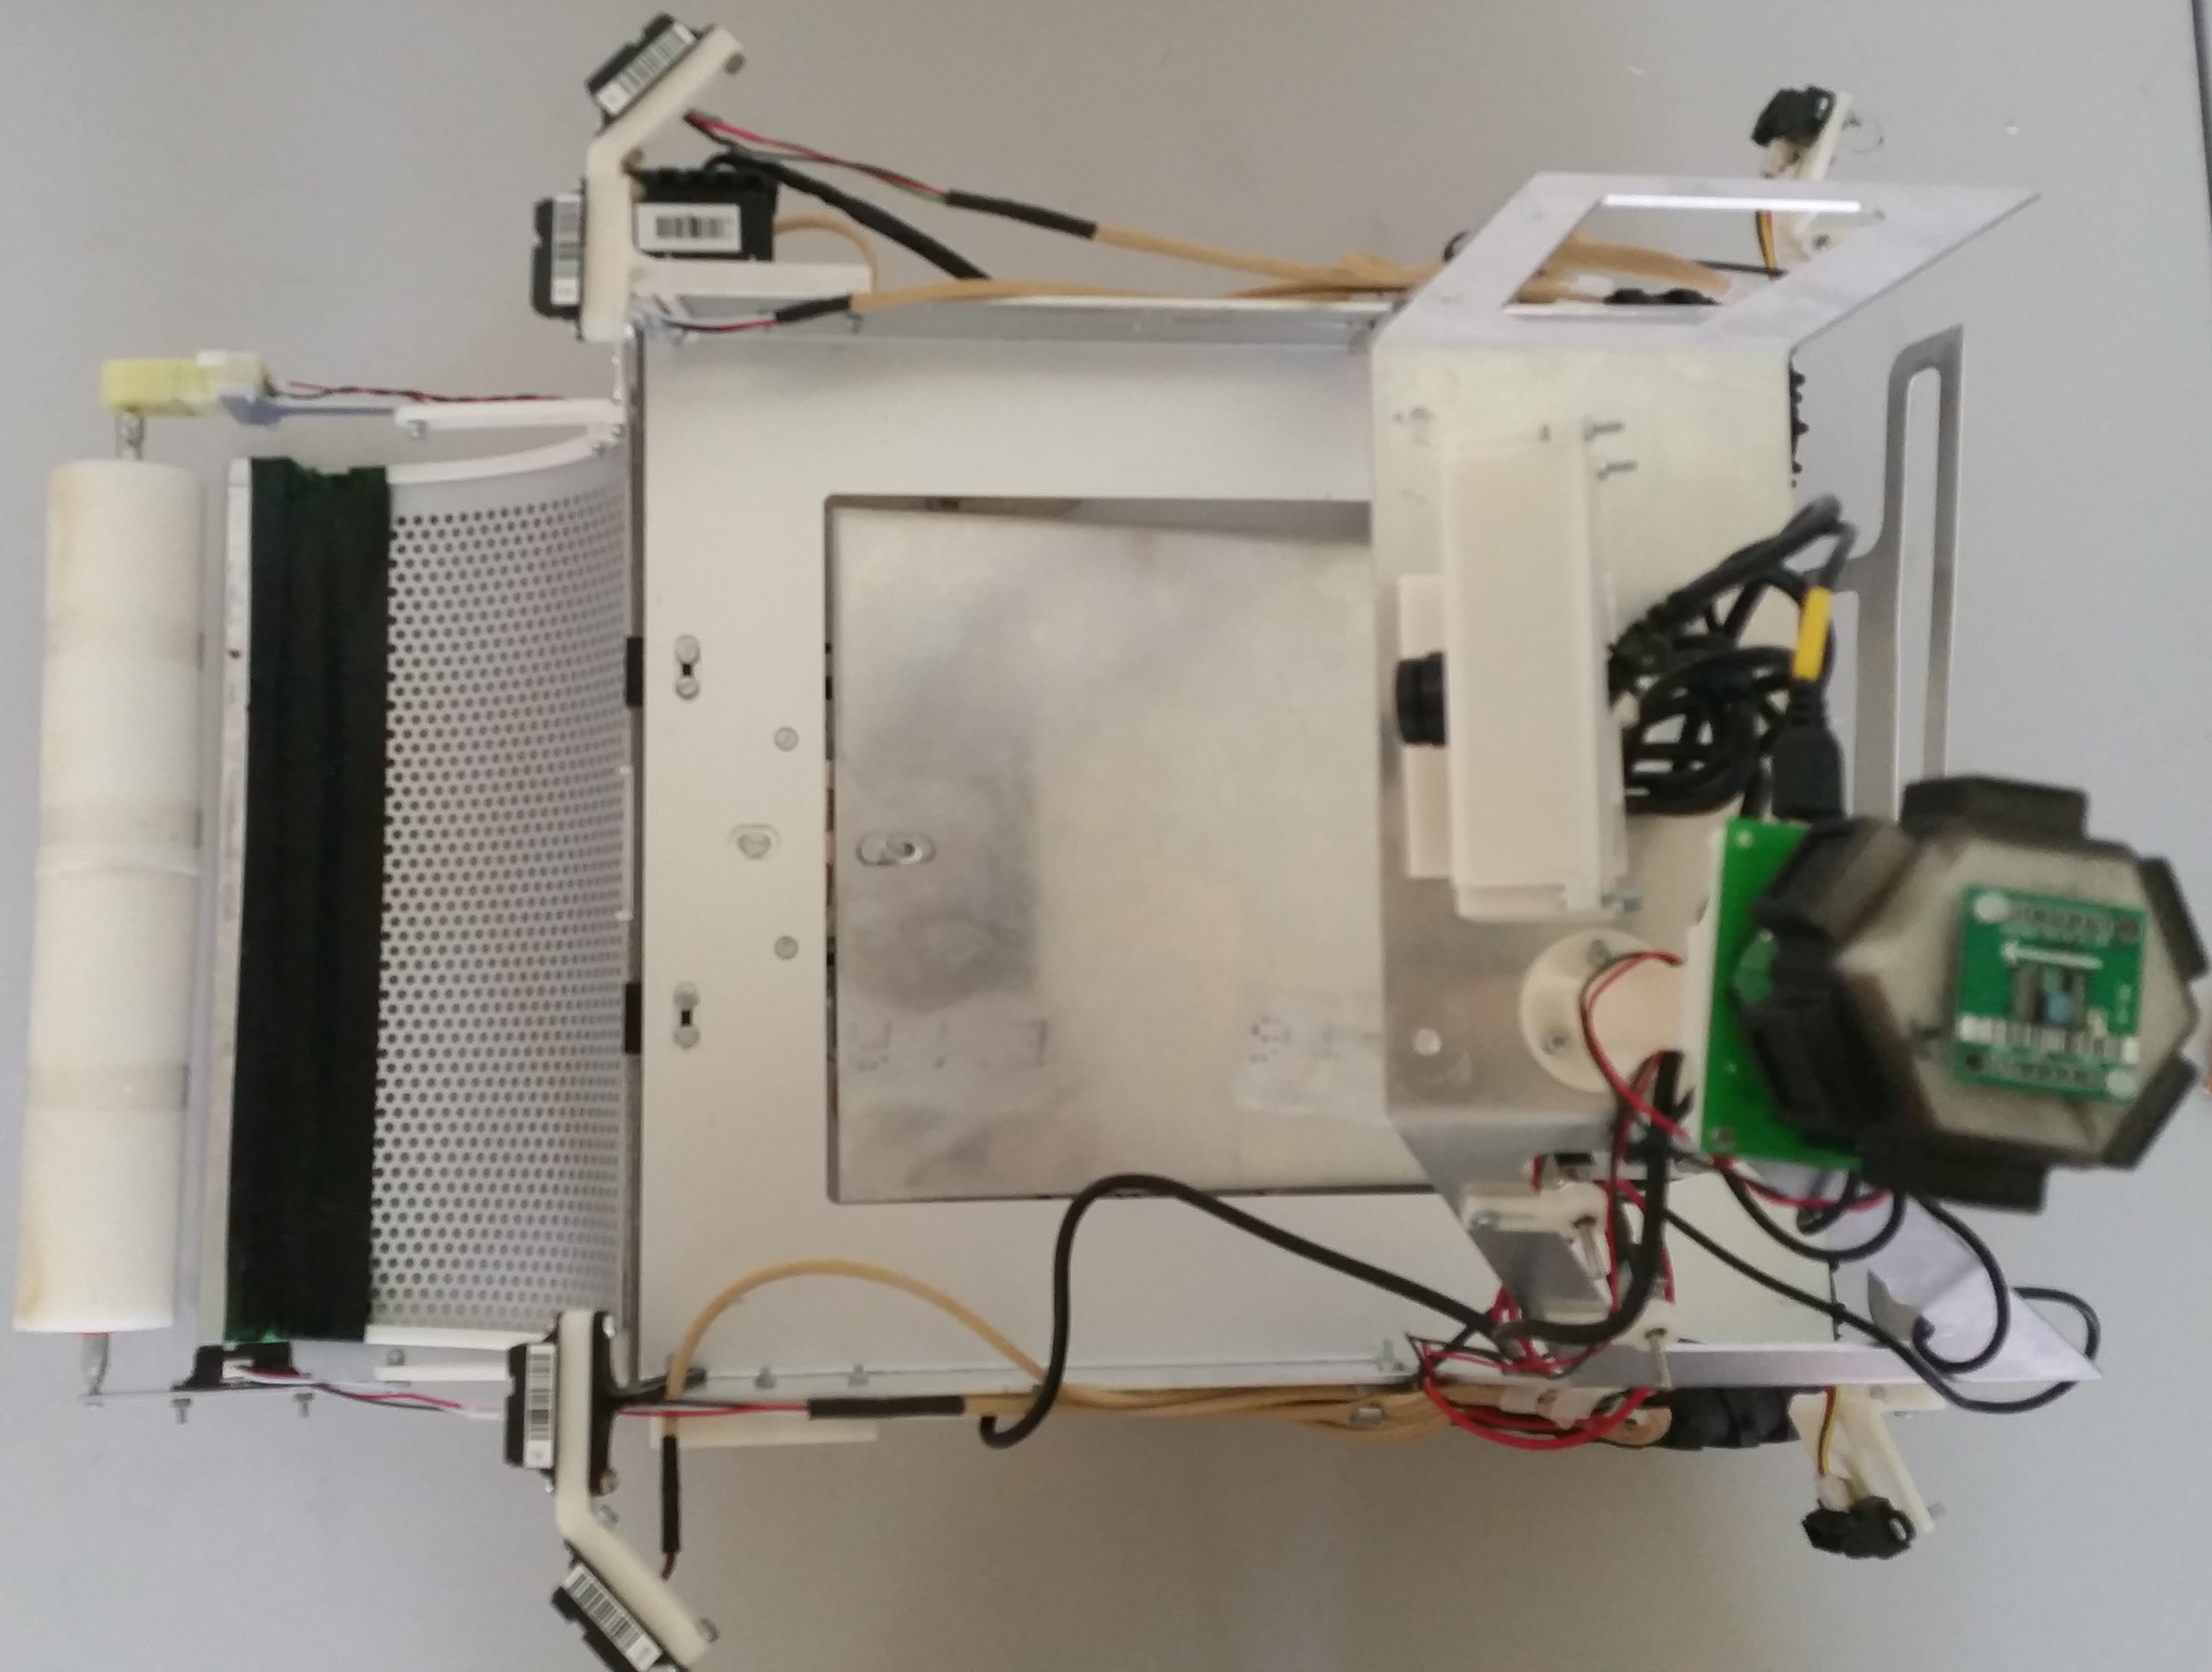
\includegraphics[width=0.4\textwidth]{robottop.jpg}
  \caption{The top view of the robot.}
\label{fig:robottop}
\end{figure}

Finally, The disposition of the sensors was changed before the competition. As in \ref{fig:robottop}, the ultrasonic sensors were removed, and 8 infrared sensors were used instead. The bottle detection worked with the camera, so the ultrasonic sensors became useless.

\subsection{Brush Motor and driver}

For the frontal brush, we needed to have a light but quite powerful motor, which could help pulling the bottles towards the inside of the robot's 'shovel'. We decided to order a $180:1, 2.2 kg\cdot cm$ motor at $4.5 volts$ bought in pololu (see Figure \ref{fig:brushmotor}).

\begin{figure}[H]
  \centering
  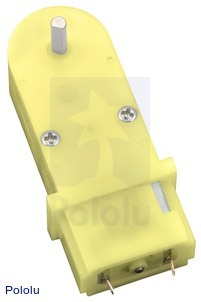
\includegraphics[width=0.2\textwidth]{brushmotor.jpg}
  \caption{A VNH5019 Motor driver Carrier.}
\label{fig:brushmotor}
\end{figure}

Agter testing this motor with bottles, we agreed on keeping it, as it was quite lightweight at a little less than 20 grams, and it worked quite well on picking up bottles. 

In order to anticipate a blocked bottle, or helping counting the number of bottles taken, a motor driver with current sense was bought, that would control the plastic motor. As the choice of motor drivers with current sense ability was quite limited, and adequate for our motor, we had no other choice than to take one that went out of the specifications recommended for the motor.

\begin{figure}[H]
  \centering
  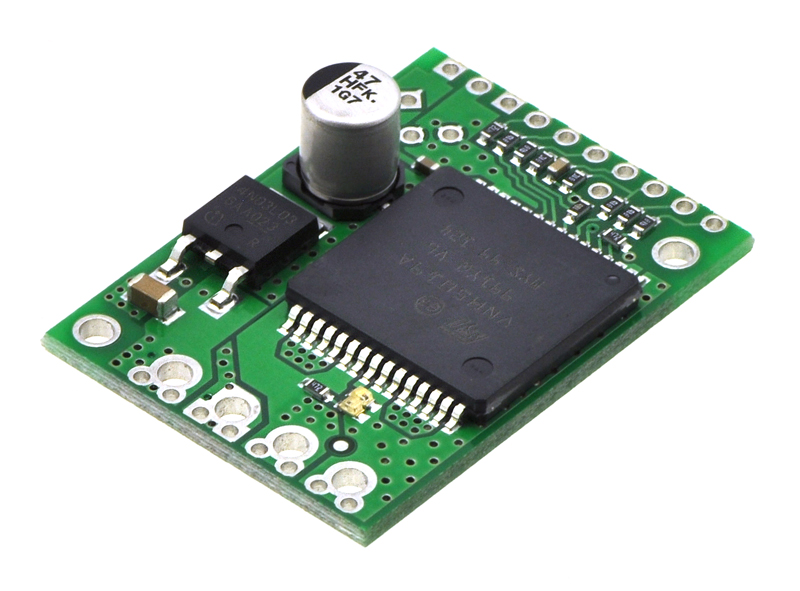
\includegraphics[width=0.3\textwidth]{driver.jpg}
  \caption{A VNH5019 Motor driver Carrier.}
\label{fig:driver}
\end{figure}

With the VNH5019 (See Figure \ref{fig:driver} above), the voltage supply was minimum $5.5 volts$, so we decided to supply the motor directly from the battery. After some research and testing, it was found that the motor works well under those conditions, if the PWM us not at the maximum. For this, the maximum average voltage supplied by the driver in PWM was kept under $4.5 V$ as recommended by the constructor.

The VNH5019 Driver for the plastic gearmotor had a current sense ability that was implemented at 140mV/A. With the arduino micro, an analog input was used to measure this voltage. At 1023 increments for a nominal voltage of 5 Volts, we can measure with a precision of $4.9 mV$ per increment. This meant that we could measure with a precision of $140/4.9 = 28 increments / Amp$, so a resolution of 35mA. As our motor had a stall current of 800mA, we judged the resolution enough for counting the bottles picked up. After some tests, we could confirm this choice as the current was clearly increasing when the bottles were being taken.

When testing this function in practice, it occured to us that the sensing data was only noise. All the wires were close to the motors, and the electromagnetic field induced false measurements. The increments were also too small to be sensed accurately, so instead we used an infrared sensor to detect the presence of bottles.

\subsection{Shovel actuaction}

For the rotating movement of the frontal shovel, the best solution was to find a servomotor powerful enough for rotating the whole shovel upwards. With a high torque of 1.5Nm, and a relatively low price, the actuator of choice was the Dynamixel smart servo (Figure \ref{fig:dynamixel} below). 

\begin{figure}[H]
  \centering
  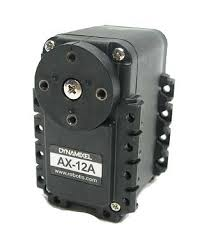
\includegraphics[width=0.3\textwidth]{dynamixel.jpg}
  \caption{An Ax-12A Dynamixel smart servo actuator.}
\label{fig:dynamixel}
\end{figure}

To supply this servo, it is recommended to use a source of 9 to 12 Volts. However, with our limited power supply it would have been needed to either switch to another power supply with higher voltage, or use a step-up voltage regulator. While testing with the arduone shield board mounted on the arduino Mega, it was observed that the smart servo didn't need that much power, and worked just fine with a power supply of 7.2 Volts. Since the board that was going to be used for the control of the dynamixel motor was not the Arduone board designed for this purpose, but the arduino micro, some modifications had to be made. Indeed, the Dynamixel actuator does not work with a full duplex serial communication protocol, but instead a half-duplex one. This means that there is only one available wire for both transmitting and receiving data. To manage to control this servo with an arduino micro, both Tx and Rx lines were connected, with a resistance of $100 \Omega$ to the Tx pin. This would prevent a short circuit from happening to the Tx pin, as the Rx pin was configured as input, and is thus protected from such a thing to happen. After this procedure, the Dynamixel worked well with 7.2 V power supply and a half duplex communication with the arduino micro.

During tests however, it was also observed that the dynamixel struggled a bit to lift the whole shovel, and since the mechanical structure of the robot was symmetric, it was possible to add a second dynamixel, connected in daisy-chain with the first one. However, the desynchronisation of the two motors, and the hyperstaticity of the assembly made them block each other, so only one motor was used. It was then not possible to lift the elevator partially.   % (\chapter{})
%\cleardoublepage
%%%%%%%%%%%%%%%%%%%%%%%%%%%%%%%%%%%%%%%%%%%%%%%%%%%%%%%%%%%%%%%%%%%%%%%%%%%%%%%%
%
%   Semester project, fall term 2014
%   Author: Jakob Ehrl, born 01/24/91
%   Study program: Computer science, MA 1
%   
%   Professor Dr. Francesco Mondada
%   Assistant: Dr. Stefan Witwicki
%
%%%%%%%%%%%%%%%%%%%%%%%%%%%%%%%%%%%%%%%%%%%%%%%%%%%%%%%%%%%%%%%%%%%%%%%%%%%%%%%%%

\chapter{Heavy duty actuation Module}

As a means of navigation, a simple yet effective choice available was to use the Wild Thumper robot chassis. This chassis was already available with motors at $75:1$ gear ratio and wheels. With a steel structure with holes every centimeter, this chassis was perfect for supporting the rest of the robot, as well as attaching different kind of modules.

\begin{figure}[H]
  \centering
  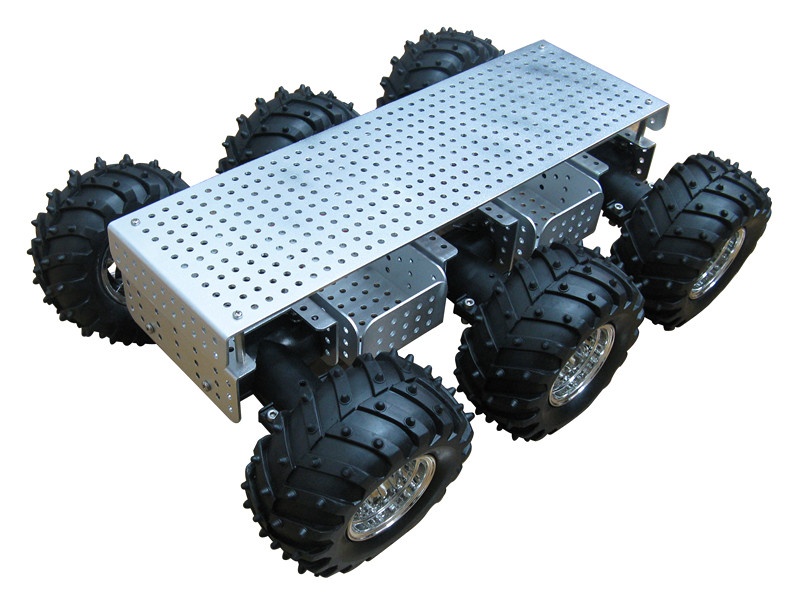
\includegraphics[width=0.3\textwidth]{wt.jpg}
  \caption{The Wild Thumper Robot Chassis.}
\label{fig:wt}
\end{figure}

After some analysing of the structure of the chassis, it was concluded that it was too long to be used for the robot. As it is a modular chassis, some parts were removed to reduce the length of the robot. At the end, only 4 out of the 6 initial wheels were implemented.

\section{Chosen Motors}

Having assembled the chassis, and the initial motors, a simple code was made, that would help test the abilities of the chassis, thanks to a soldered remote controller.\\

(((((((((((((((((( FIGURE of the controller)))))))))))))))))\\

The chassis was functionnal, however, it was lacking some torque already, and it was empty, and maybe too fast. Another problem was that with the newer configuration in which it was built, the wheels were drifting when the robot was attempting to rotate. This was a problem, because on a rough surface such as the one of the competition, the torque would not be high enough to allow the robot to rotate.\\

Some precautions were taken in order to remedy to this problem:\\

Firstly, the motors were changed to ones with a higher gear ratio $(172:1)$ to allow the wheels to have more torque.\\

Secondly, the ones with encoders were purchased, for safety measures, as it could always be useful in the future, and not a problem if they are not used. \\

Thirdly, in order to reduce friction during the rotations, the front wheels were replaced with 3D printed cylinders. The rear ones had the encoders, and need to drift the minimum possible. \\

\begin{figure}[H]
  \centering
  \includegraphics[width=0.3\textwidth]{wheel.jpg}
  \caption{The 3D printed wheel, in comparison with a Wild thumper default wheel.}
\label{fig:wheel}
\end{figure}

%\textbf{And Lastly, a non-holonomic algorithm for the trajectory planning of the robot was implemented, so %that the robot would be able to move and rotate at the same time, reducing the stress on the wheelss.}

\section{Feedback speed Control}
A driver for the wild thumper was written, with the ability to count the pulses received from the encoders. However, as a replacement solution was found, the encoders were not used for the robot navigation.

\section{Tailgate}

To control the tailgate of the robot, in order to unload the bottles, a servo coupled to an aluminum plate was installed. 
As a Dynamixel AX-12A Smart servo was too powerful, we prefered to use a standart servo for this task.

\begin{figure}[H]
  \centering
  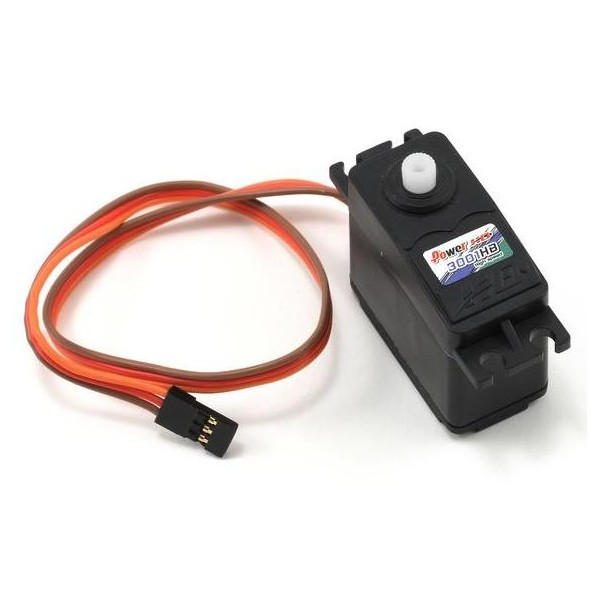
\includegraphics[width=0.3\textwidth]{servo.jpg}
  \caption{The 3001HB Servomotor.}
\label{fig:servo}
\end{figure}

With a torque of $4.4kg \cdot cm$, the 3001HB was the perfect servo for this task. As the torque needed was used only for the unloading of bottles, and the only stress on this motor was the gravity force of the bottles. 

The 3001HB serves perfectly it's purpose and has just the right amount of torque needed.

\section{Tests}

The testings were done in the beginning with the remote control, and later on with the wireless laptop control implemented on the Odroid. With the first tests a conclusion was made that the 75:1 gear motors were not powerful enough. Later with the higher gear ratio, the robot was slower but could move in an easier manner. On the grass, where the maximum friction, the robot was struggling to rotate, because of the position of the wheels, and the affected friction. After changing the front wheels with plastic cylinders, the robot could turn with ease, and no negative impact was found.    % (\chapter{})
%\cleardoublepage
%%%%%%%%%%%%%%%%%%%%%%%%%%%%%%%%%%%%%%%%%%%%%%%%%%%%%%%%%%%%%%%%%%%%%%%%%%%%%%%%
%
%   Semester project, fall term 2014
%   Author: Jakob Ehrl, born 01/24/91
%   Study program: Computer science, MA 1
%   
%   Professor Dr. Francesco Mondada
%   Assistant: Dr. Stefan Witwicki
%
%%%%%%%%%%%%%%%%%%%%%%%%%%%%%%%%%%%%%%%%%%%%%%%%%%%%%%%%%%%%%%%%%%%%%%%%%%%%%%%%%

\chapter{Localization Module}
The localization module is composed of an arduino micro, 6 linear sensor arrays, and a compass. Mounted on a rod in a high position on the robot, it's purpose is to use the geometry of the map, the beacon peaks received by the linear sensor arrays, and the orientation read from the compass in order to triangulate the position and orientation of the robot in the map.

\begin{figure}
\centering
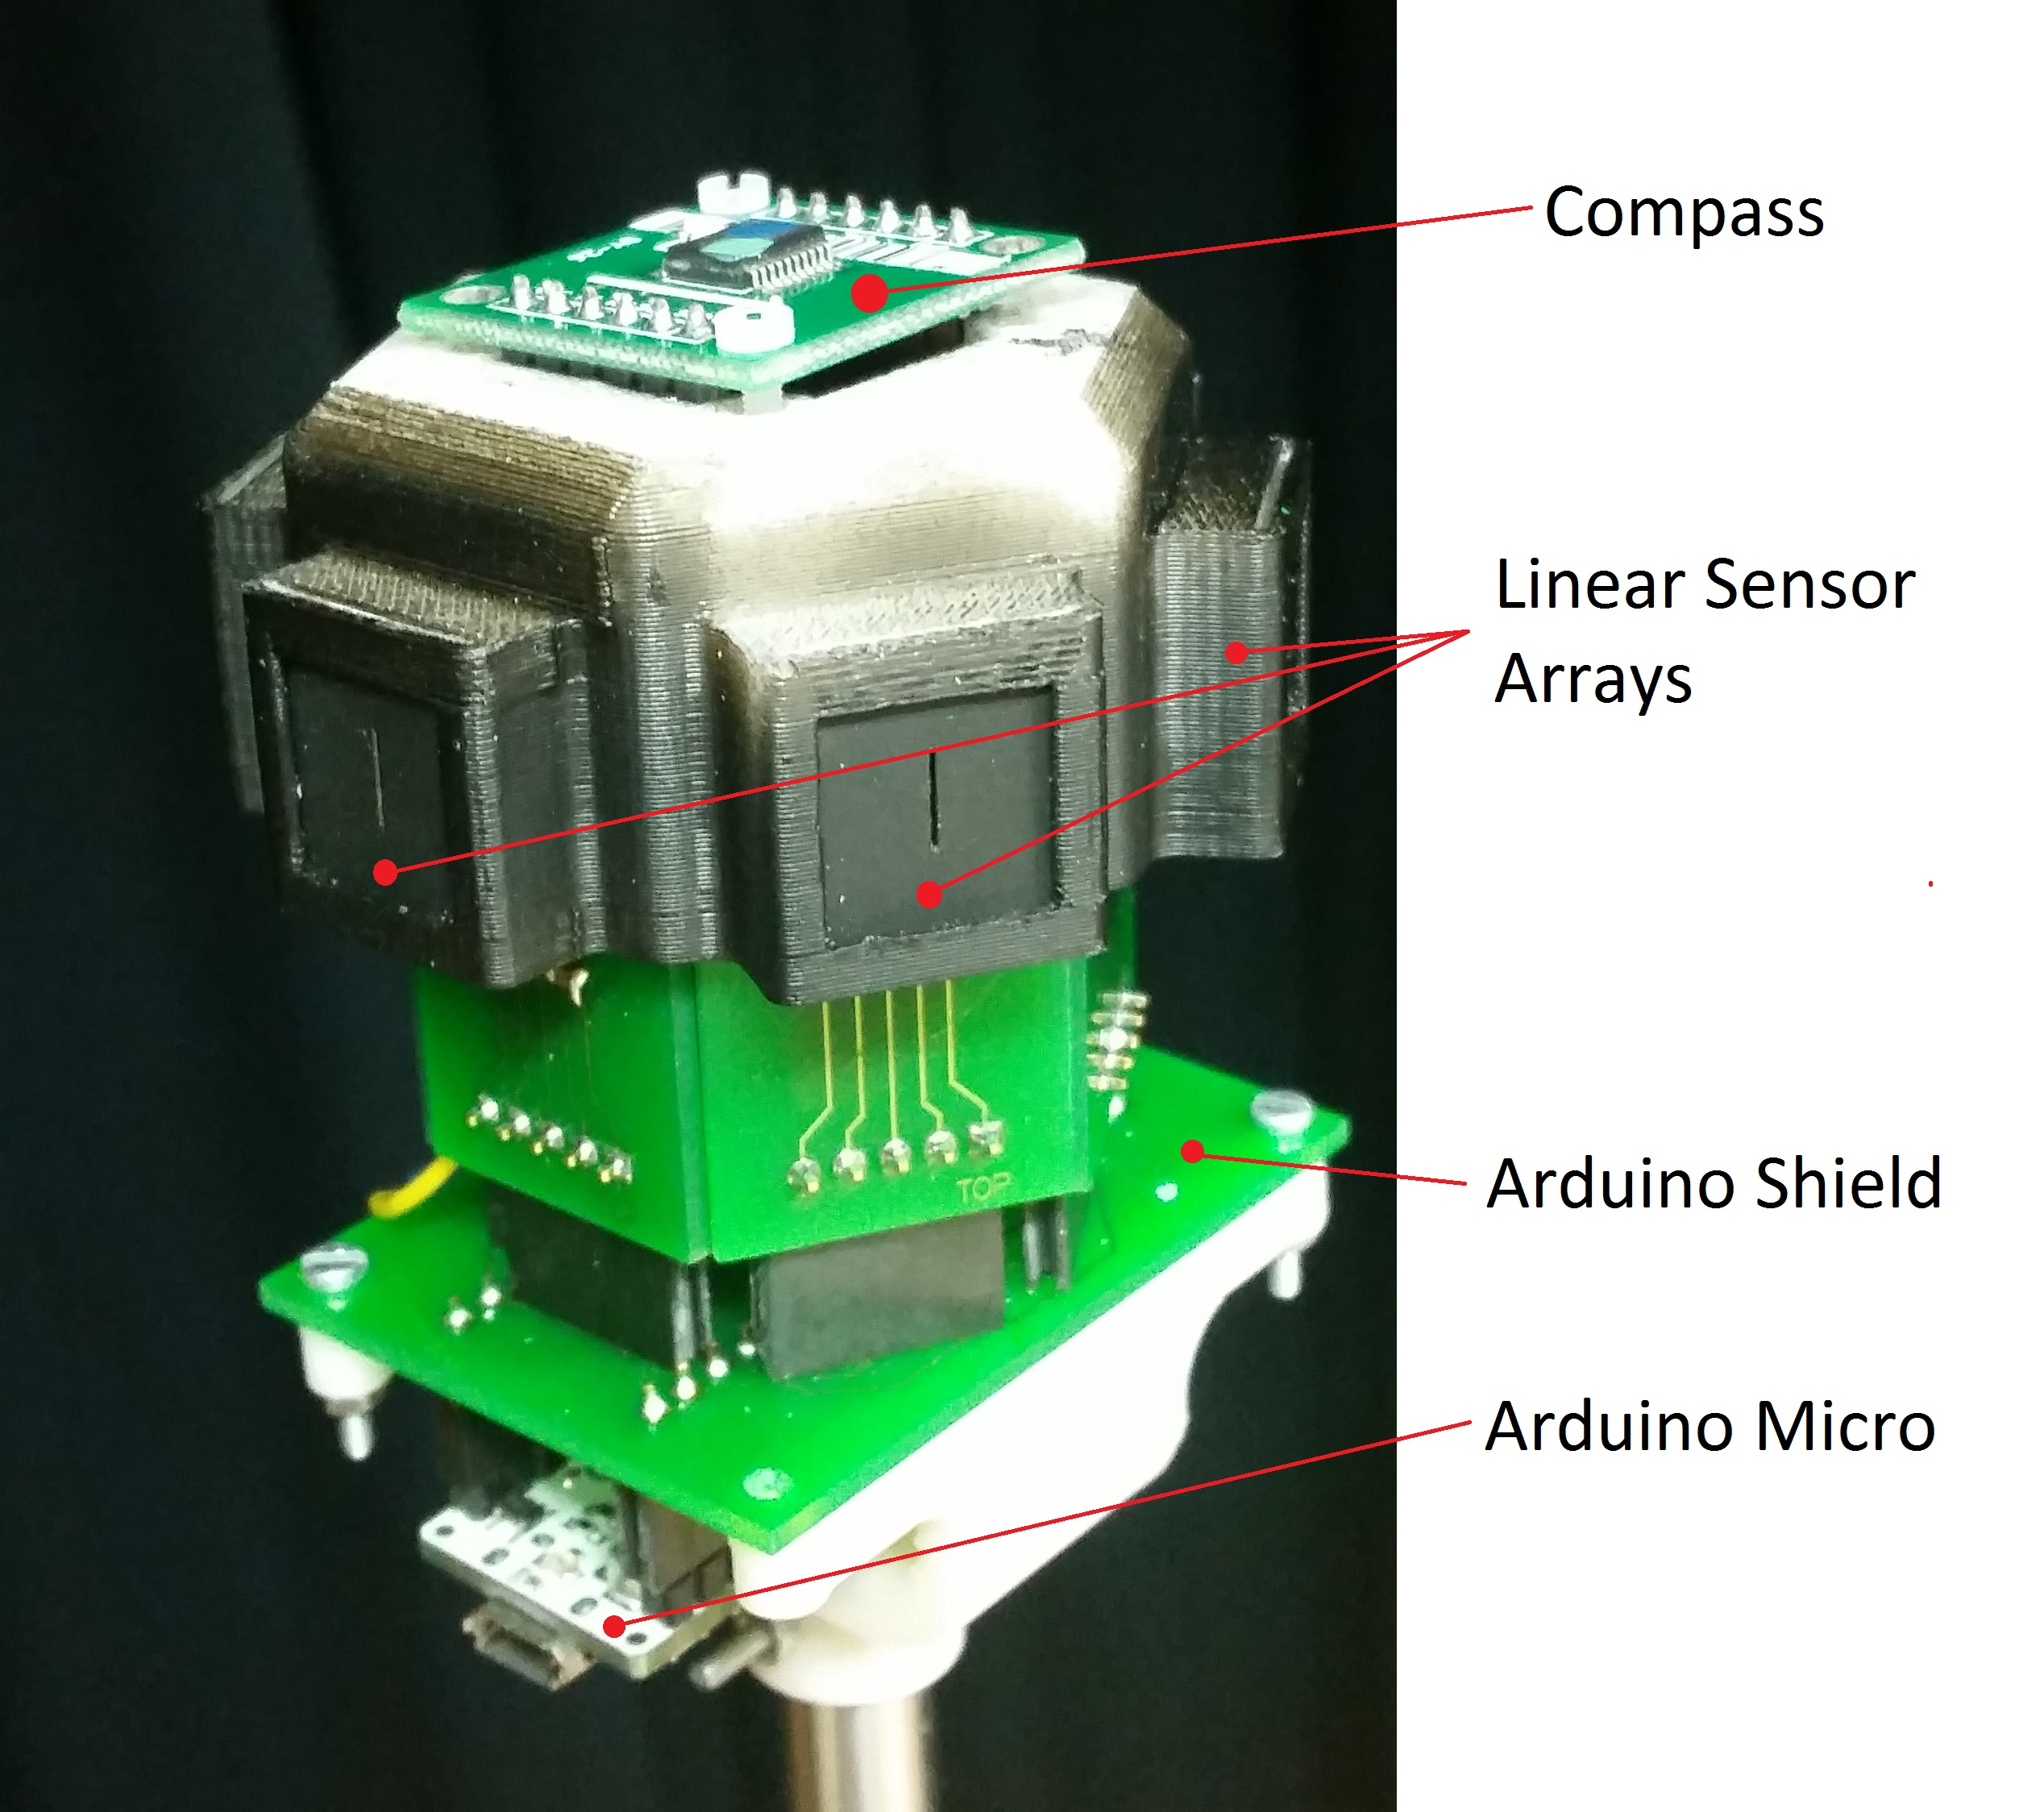
\includegraphics[width=0.5\textwidth]{lincam.jpg}
\caption{The localization module.}
\label{fig:lincam}
\end{figure}

\section{Sensors}
Data from two different sensor types are fused to obtain the robot's pose 
(position and orientation) in the arena. A digital compass and an array of
six linear cameras

\subsection{Compass}
The compass directly returns the orientation in a range from $0.0^\circ$ and $360.0^\circ$.
Pose updates are queried once per iteration. The purpose of this sensor is to 
give absolute orientation estimates in any place of the arena and independently of
occlusions. In the arena, the compass was also calibrated at the initialization of the program, in order to have a fixed north, pointing at the robot starting orientation.

\subsection{Linear Cameras}
The heart of our localization module is formed by six linear cameras arranged 
as a hexagon. All pixel arrays have the same height and inclination, which allows
us to make the simplifying assumption that an image stitched together from all the
cameras captures a $360^\circ$-scene and can be mapped to a circle. Missing pixels
in gaps between, cameras and also the fact that the arrays are not exactly circular
but piecewise planar, are ignored in the following.

Given that there are four light beacons attached to the corners of the arena a 
2D position can be computed from the intensity peeks in the camera image.
This setup could technically be used as a standalone module to determine orientation
and position even without compass (if an initial pose is known). However, a compass 
adds valuable redundancy and especially allows for accurate orientation measurement
in any location inside the arena whereas the achievable accuracy of triangulated 
values through the camera signal varies strongly within the arena due to occlusions
or distant light beacons.

\section{Localization algorithm}
Each camera is equipped with a linear image sensor of length 102 and depth 255. This
yields a total of 612 pixels on the whole circle. Mapping pixels to degrees causes a 
resolution of approximately two pixels per degree. An exact determination of peeks 
representing the four light beacons is difficult for two main reasons: firstly, there may be
reflections causing false negatives and secondly, there will be at most three beacons
seen at a time since the fourth one is occluded by the elevated zone of the arena.
Both cases cause ambiguities that would have to be resolved in a bottom-up approach
where one tries to infer position from image peeks. To deal with this difficulty,
we designed a top-down algorithm that follows the idea of expectation maximization.

General:
\begin{itemize}
    \item coordinate origins are in the corner of the recycling zone
    \item global orientation of arena is known (rotation of coordinate systems
        between localization module and arena is determined by compass)
\end{itemize}

In a prior consideration, the arena is divided into equally spaced squares. The area
of $8m \times 8m$ is sub-sampled in steps of $0.5m$, giving $15 \times 15$ discrete 
positions (walls are excluded). For this limited number of points, we pre-compute 
the expected position of beacon images in the pixel array. The result is stored in
\texttt{char prior[15][15][4]}. Dimensions one and two refer to the $x$- and $y$-coordinates.
The third refers two the beacon index.

Consider Algorithm~\ref{alg:localize}. Instead of searching for peeks in the signal 
and estimating our position by triangulation,
we reduce location updates to a weighted average of four pre-computed sampling points.


\begin{algorithm}
\caption{Position update.}
\label{alg:localize}
\begin{algorithmic}[1]
    \Statex Given: initial position $\vec{p_t} = (x_t, y_t)$, camera image $I$, prior[x][y][idx], mapping from angle to pixel index
    \Statex compute new position $\vec{p_{t+1}}$ as
    \Statex 
    
    \State $\theta \gets$ angular measurement from compass
    \Statex

    \Statex determine current tile and use known sampling points
    \State $\vec{s_{00}} \gets (x, y)$ of left, bottom
    \State $\vec{s_{10}} \gets (x, y)$ of right, bottom
    \State $\vec{s_{11}} \gets (x, y)$ of right, top
    \State $\vec{s_{01}} \gets (x, y)$ of left, top
    \Statex
    
    \Statex compute weights of neighboring samples given the actual intensity response as
    \ForAll{$\vec{p_{xy}}$} 
        \State $w_{xy} = \sum_{i = 0}^4 I(prior[x][y][i] + angleToPixel(\theta))$
    \EndFor
    \Statex 

    \Statex new position as weighted average of known samples
    \State $\vec{p_{t + 1}} = \frac{w_{00} \cdot \vec{s_{00}} 
            + w_{01} \cdot \vec{s_{01}} 
            + w_{11} \cdot \vec{s_{11}}
            + w_{10} \cdot \vec{s_{10}}}
            {w_{00} + w_{10} + w_{11} + w_{01}}$ 

\end{algorithmic}
\end{algorithm}

Given an initial position, we know which sampling points to consider. The prior
tells us where to expect peeks in the image signal. Sample points gain more impact
on pose estimates if they match the expectation more, i.e. have high intensity values 
close to the predicted indexes of beacon images. Knowing an approximate location
lets us rule out all ambiguities that might arise from occlusions or false positives.
A pre-processing step where the circular intensity signal is convolved with a box
filter (sliding average) will widen the peeks and thereby make predictions more
reliable. If the peeks were too distinct and close to Dirac impulses our prior 
is more likely to fail.

\begin{figure}[H]
\centering
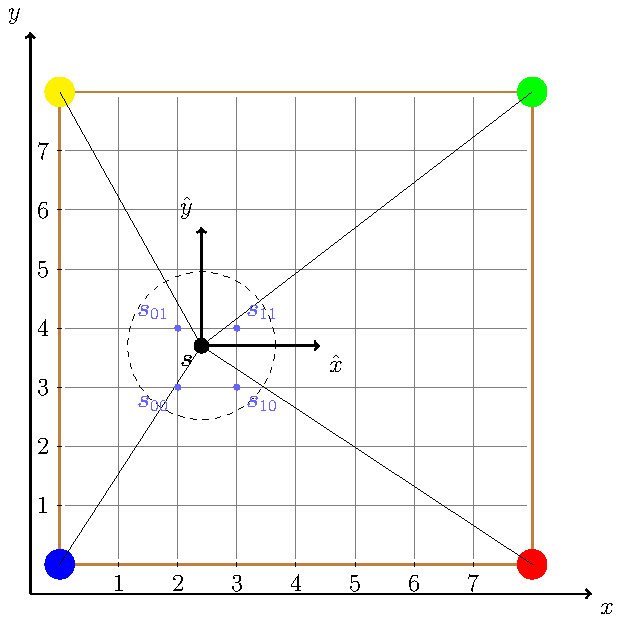
\includegraphics[width=0.5\textwidth]{figures/fig_localization_grid.pdf}
\caption{Exact location $\vec{s}$ and the four closest sampling points. Robot coordinate system is aligned with the arena (no rotation).}
\label{fig:localization_grid}
\end{figure}

% TODO place somewhere else in text
Figure \figurename~\ref{fig:localization_grid} shows the four beacons in the corners of the map, the coordinate system used, and the robot's position.

We want to determine the robots exact
location $\vec{s}$. From previous measurements, we know that we are in the tile
bounded by $\{\vec{s_{00}},\vec{s_{10}},\vec{s_{11}},\vec{s_{01}}\}$. For each 
neighboring sample point, we find the intensity values at the pixel indexes 
predicted by this point (check prior at $\vec{s_{ij}}$ for the needed pixel indexes).
For each $\vec{s_{ij}}$ we then receive a vector of four intensity values. 
Based on the intensities, we compute weights for each sample point. A weighted 
average of  $\{\vec{s_{00}},\vec{s_{10}},\vec{s_{11}},\vec{s_{01}}\}$ yields the
final location estimate.
Note that if we are 
close to a sample point then the respective intensities will be higher because the
peaks match the prediction more than if we were further away. Also if a beacon is
occluded, its respective response would be equally low at all the neighboring  
positions. Hence, we can ignore this fact.
The orientation $\theta$ is important to rotate the local coordinate system before
applying the prior, i.e. the predicted peak pixels must be shifted.

In a very abstract manner 
\begin{itemize}
    \item the prior stores angles at which we expect peaks (as pixel indexes)
    \item the compass is needed to rotate/shift the angles from the prior correctly
    \item we sum up over intensities at indexes given by the prior
    \item this gives us a notion of ``how much does the current location match the predicted one''
    \item weighting the nearest neighbor sample points will give a more accurate
    position estimate
\end{itemize}



\section{Tests}

In order to visualize the readings of the different sensors, and to test the algorithm performance in the arena, a python script was written. The script shows a visualization of the intensity values of the 612 pixel array obtain by combining the 6 linear cameras. The blue arrow is also the direction obtained by reading the compass.
 before having the arena, we tried visualizing the peaks in ``good'' conditions. In figure \ref{fig:goodpeak}, the peaks are very high, and easily visisble. 

\begin{figure}[H]
\centering
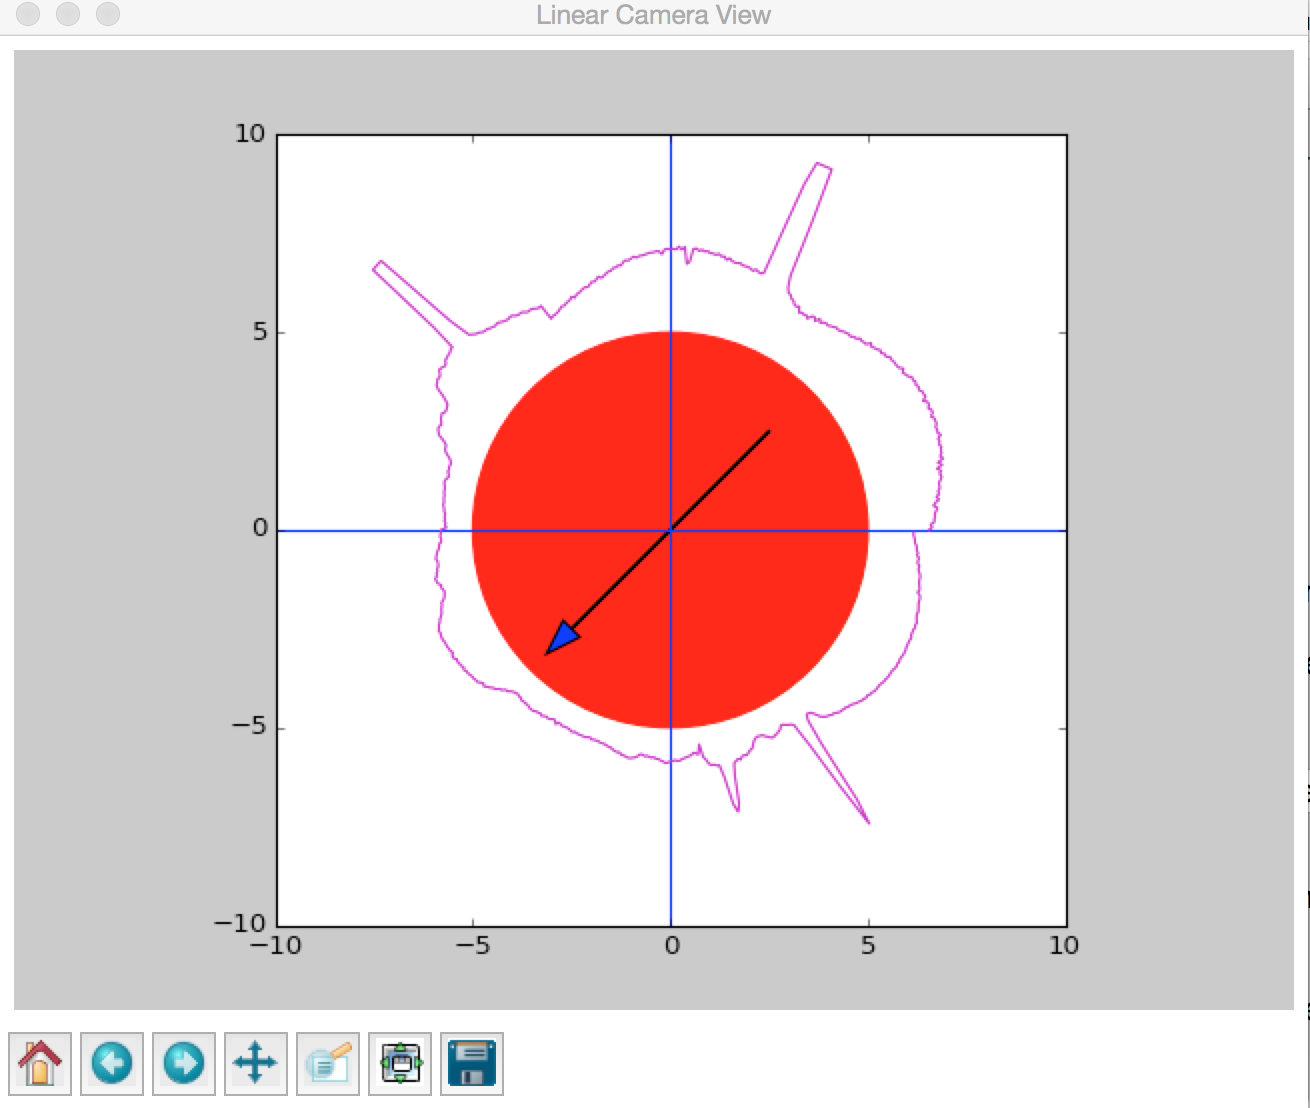
\includegraphics[width=0.5\textwidth]{goodpeak.png}
\caption{Data aquired from the linear sensor arrays in optimal conditions ( low ambient light, high beacon intensity).}
\label{fig:goodpeak}
\end{figure}

With such good conditions, it is easy to find the position of the robot. However, in the real arena, the results were slightly different. In figure \ref{fig:peak}, the real results are shown. As it can be observed, the peak with the highest intensity is coming from one beacon. In this diagram, the robot is very close to the starting position, this is why the intensity is so high. However, the other beacons are barely visible. Some steps can also be observed in the graph, and corresponds to some imperfections of the linear sensor arrays. The sensors were soldered by hand and may not be perfectly flat on the PCB.

\begin{figure}[H]
\centering
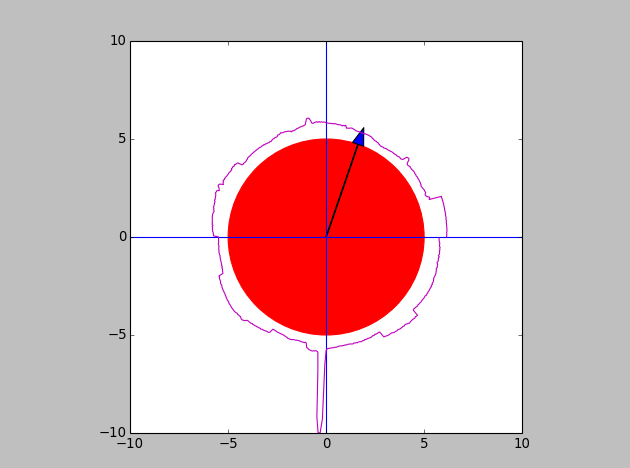
\includegraphics[width=0.5\textwidth]{peak.png}
\caption{Data aquired from the linear sensor arrays in the arena (high ambient light, low beacon intensity).}
\label{fig:peak}
\end{figure}

In the last figure (Figure \ref{fig:roof}), multiple peaks with very high intensity can be seen. These ones corresponds to the roof lights, which are very far. Just by tilting slightly the sensors, ligh pollution begins to appear quite quickly.

\begin{figure}[H]
\centering
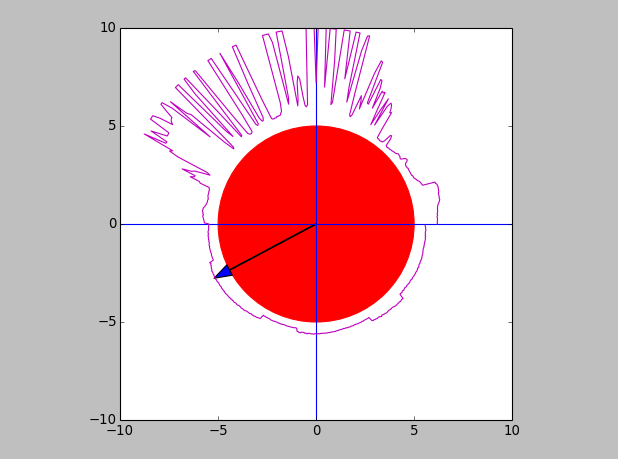
\includegraphics[width=0.5\textwidth]{roof.png}
\caption{Data aquired from the linear sensor arrays in when aiming at the roof of the arena.}
\label{fig:roof}
\end{figure}   % (\chapter{})
%\cleardoublepage
%%%%%%%%%%%%%%%%%%%%%%%%%%%%%%%%%%%%%%%%%%%%%%%%%%%%%%%%%%%%%%%%%%%%%%%%%%%%%%%%
%
%   Semester project, fall term 2014
%   Author: Jakob Ehrl, born 01/24/91
%   Study program: Computer science, MA 1
%   
%   Professor Dr. Francesco Mondada
%   Assistant: Dr. Stefan Witwicki
%
%%%%%%%%%%%%%%%%%%%%%%%%%%%%%%%%%%%%%%%%%%%%%%%%%%%%%%%%%%%%%%%%%%%%%%%%%%%%%%%%%

\chapter{Central Processing}

\section{Setup of Processing Units}
Our robot is equipped with four different processing units that, together,
form a network of workers performing individual tasks. There is one master
node that receives sensor readings and lower level computation results from
the other nodes. This data is used to make decisions and finally send 
commands to control the actuators.


\subsection{Master Node}
An Odroid-C1 was used as master node. Similar to the well known Raspberry Pi,
this miniature computer has a Unix-based operating system and possesses numerous
ports such as USB, Ethernet, HDMI and various GPIO pins. We decided to use this
board instead of the Raspberry Pi, which is available in the virtual catalog,
because of the way we intended to design the network of processing units and 
data processing. With four USB ports instead of only two, four CPU cores and twice 
the amount of SDRAM, the Odroid-C1 allows to easily connect the other processing 
boards as well as a camera via USB. This allowed us to develop code in the same
way as if we were working on usual desktop computers. The need for a quad-core 
processor is justified since we aimed at separating the software into different 
modules that are supposed to run independently and in parallel. Pthreads were
used to process data from different inputs independently instead of in a single-loop program.

\subsection{Slaves}
Three Arduino boards were connected to the odroid via serial connection. The following
lists their responsibilities.

\begin{itemize}
    \item Arduino Micro 1
    \subitem control of brush motor
    \subitem data acquisition from five infrared sensors
    
    \item Arduino Micro 2
    \subitem data acquisition from compass 
    \subitem data acquisition from linear cameras

    \item Wild Thumper Controller
    \subitem control of wheels
    \subitem control of tailgate
\end{itemize}

\subsection{Communication}
To transmit data acquired by the Arduino boards and commands generated by the master,
we use the serial communication protocol. The micro controllers do not communicate with
each other. On both sides of the transmission there is a timed control loop that reads
and writes data at a frequency of 30 Hz. To reduce communication costs, all the available
data is first stored in a buffer. Only one message with all the collected commands/sensor
readings is transmitted per interval. This also allows us to filter sensor readings
and reduce communication overhead when the micro controller's control loop is faster 
than the master's planning phase.

\subsubsection{Message Format}
A message is composed of four ASCII characters. The first character being either an
upper- or lowercase character and the following three characters being digits with
leading zeros. Uppercase letters denote command IDs while lowercase letters denote
sensor IDs. Any number between 0 and 999 is allowed as respective value. 

\subsubsection{Limiting Factors}
Since Arduino boards have a small buffer for serial communication (64 bytes), continuous
communication causes a major bottleneck on the micro controllers. Therefore we 
had to limit the update frequency to 30 Hz and also limit the number of messages
that can be sent per iteration.


\section{Master Program Structure}
Code for the master node was written in C++ and designed in a modular way. The bottom
layer includes modules for sensing and acting. A middle layer provides easy access to 
the most recent sensor readings and also an interface for high-level control functions
by hiding actual actuator IDs and value checks behind human readable names such as
\texttt{setWheelSpeeds\{left, right\}}. The top level is where plans are made and 
commands are created. It offers both human interaction via keyboard or autonomous mode
through implementation of classes with access to the middle layer.

\subsection{Bottom Layer}

\subsubsection{Communication Module}
The class \texttt{Serial} implements low level serial communication between the master
node and any other node. The command line options \texttt{ard1, ard2, wtc} specify 
which entity the object shall represent. Their respective serial port locations must
be given as arguments after the option. For testing purposes, the program can be run
with three, two or no slave node connections.

Each connection to a slave is bounded in an object of class \texttt{Serial} having 
its own read and write buffer and its own thread. The communication loop inside a thread
is timed to read and write data at a frequency of 30 Hz to be congruent with the
micro controllers.

\subsubsection{Vision Module}
The class \texttt{Detector} implements the vision part of the robot. An object of this
class can be created from a connected camera or a single image (for development purposes).
It offers two options for image processing both working with color images. 

The first algorithm is based on a K-Means segmentation of the image. \texttt{BGPattern} allows
to create a desired number of color patterns that are later used to segment the image
into background and foreground. Given that there is a very limited number of possible
backgrounds in the arena (tiles, wood, grass, stones), the basic idea was to assign 
pixels within a certain distance to one of the background patterns. Pixels that are too
far from any of the clusters could then be considered as candidates for bottles.
Morphological operations (opening for noise reduction and dilation for region growing)
on the remaining binary image would eventually allow to classify regions of a certain
size and shape as bottles or obstacles.

The second algorithm is also based on the assumption of highly uniform background
patterns. It is implemented by the class \texttt{RangeFinder}. Assuming that the robot
is currently on drivable terrain, a small area in the lower part of the image (directly
in front of the robot) is used as sample pattern. This region is extended toward the
top of the image whilst the change in color is below a certain threshold. Boundaries
of this area are candidates for obstacles, bottles or sudden terrain changes. This 
option was found to generalize better than the first. A more detailed description is
given in the next section.

\subsection{Middle Layer}
The class \texttt{Brain} serves as a wrapper for sensing and acting modules. It 
communicates with objects from the bottom layer (\texttt{Serial, Detector}).
It provides access to all the measurements via the respective IDs defined in \texttt{defines.h}).
Getter and setter functions with respective value range checks allow to use the low-level 
functions from a more abstract point of view.

\subsection{Top Layer}
In order to control the robot either manually or from a custom controller, it is 
necessary to create objects from the lowest level and instantiate an object of type \texttt{Brain}.
An example for keyboard control can be found in \texttt{main.cpp}. Keys are directly mapped
to actions and therefore allow for remote control. Displaying visual output is optional
and can be disabled by the option \texttt{no\_cam}.

For autonomous mode, we tested two different approaches in the classes \texttt{Simulation} and
\texttt{Autonomous}.

\section{Vision}

\subsection{Camera}
A Playstation 3 Camera, an off-the-shelf USB camera, was mounted on a bridge on top of 
the robot covering a field of view from 10~cm to 250~cm in front of the robot and 
widths of 50~cm to 280~cm respectively. This camera was mainly chosen for its easily
modifiable Linux driver and its wide range of manual options such as exposure time,
gain and frame rate. Short exposure times at a constantly high frame rate were needed
to avoid blurred images. Since the camera is mounted almost 50~cm over ground, vibrations
and rough terrain (rocks) might cause blur and thereby make images useless.

\subsection{Algorithms}
Images taken by the camera were not only processed for object detection but also for 
the detection of terrain changes. Since our robot's bottle collection mechanism can only
work when it touches the ground, approaching the grass area or the rock barrier are
a particular danger causing the shovel to hook under the grass carpet or a rock.
The following explains the three key parts of our final algorithm.

\subsubsection{Preprocessing}
The input image is a $320 \times 240$ RGB image. 
An integral image is created from the original frame. Colors are not transformed into
gray scale. Therefore, the resulting integral image is still a three-channel matrix
of size $width + 1 \times height + 1$. The main advantage of integral images is 
that sums over rectangular pixel areas can be computed in constant time. The later
steps take advantage of this fact when computing average colors or applying filters.

\subsubsection{Terrain Segmentation}
Assuming that the image bottom captures drivable terrain, we want to grow determine 
future drivable terrain by growing the region captured in the image bottom toward
the top of the image.

For this purpose, the image is divided into 16 equally spaced columns of 20 pixels width.
In each column, we compute the average color over a region of 20 pixels height, hence 
a block size of $20 \times 20$ pixels. We then move up the image by half a block size
and re-compute the average color. We repeat this step until the distance between the
current and the preceding (half a block size lower) region is above a certain 
threshold. From an abstract point of view, we grow the drivable area by allowing a 
limited change in color. \figurename~\ref{fig:segmentation} shows the robots's point
of view when approaching the elevated area. For visualization the image is masked
with the result of the terrain segmentation step. Black means non-drivable.

Initially, we were planning on having a travel mode where the robot would move with the 
shovel slightly lifted. In order to still produce a good terrain segmentation,
we built in a mask that checks for the height of the white (high intensity) brush
in the image and consequently allows for vertical offsets of the central ten bars.

\begin{figure}
\center
\subfigure{
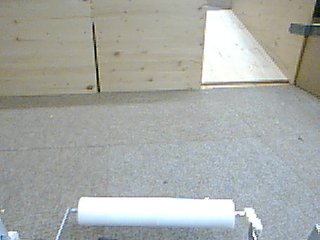
\includegraphics[width=0.45\textwidth]{figures/005.png}}
\hfill
\subfigure{
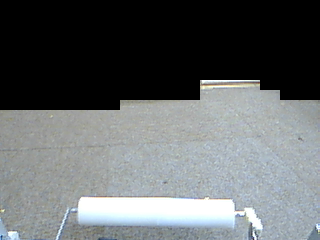
\includegraphics[width=0.45\textwidth]{figures/005-mask.png}}
\label{fig:segmentation}
\caption{Segmentation of drivable terrain.}
\end{figure}

\subsubsection{Detection of Terrain Transitions}
Given that terrain transitions in the arena are sharp straight lines, we can detect
those by fitting a regression line to the result of the segmentation step. Mostly, the
next encountered terrain does not span over the whole image and also only a small portion
of it is interesting to the robot -- the portion directly in front -- since it cannot
displace itself laterally.

Using OpenCV's \texttt{fitLine} function, we estimate a line in
2D over the central ten column heights of the previous step. Using the resulting
slope and offset, we compute the mean squared error of our estimate (summing up the 
squared differences between the true column heights and the predicted ones).
\figurename~\ref{fig:transition} shows the robot's point of view when approaching the
rock barrier with the expected terrain boundary denoted by the regression line in blue.

\begin{figure}
\centering
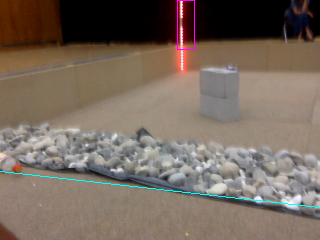
\includegraphics[width=0.45\textwidth]{figures/terrain-transition.png}
\label{fig:transition}
\caption{Regression line to terrain segmentation.}
\end{figure}

A low error means that the line fitting is appropriate and a terrain change is likely
while a high error signalizes a noisy boundary of the field of view. Boundary interruptions
(some columns lower than others) can be caused by obstacles, bottles or difficult lightning
conditions. Distance measures from the camera can help to detect 
terrain transitions as they cannot be seen by the infrared sensors. Obstacles,
however, can be detected by the infrared sensors. Consequently, range data from 
our infrared sensors should have higher weight then vision data and vision data
shall be used in cases where we have no response from infrared sensors.

\subsubsection{Beacon Detection}
Also seen in \figurename~\ref{fig:transition} is a purple frame around the light beacon.
Beacon detection can be handled in a very simple manner if the color does not need
to be determined. In our case, we decided to restrict to the pure detection without 
color classification since only the yellow beacon in the recycling zone was important
for our strategy. Having the compass and the information that there exists a beacon
in the current image, we can determine the corner we are approaching.

In our camera setup, beacons do always intersect with the upper image boundary.
We can therefore detect beacons by convolving the upper part of the image with a top-hat filter
moving from left to right. The pixel column with maximal response is considered a beacon
if its response exceeds a certain threshold in one of the three color channels. The filter
window height spans 20 pixel rows and 20 columns (5 negative columns on each side and 10 for
the central positive part). Taking the average over multiple image rows guarantees
that beacons are detected even though their intensity is not constantly high (due 
to the interruptions between LEDs). 

Once a tentative beacon column is found, the filter moves downward in the image.
In order to account for tilted beacons (or the camera not being mounted perfectly
horizontally), we allow for a small lateral motion of the filter window to the left
or right.

\subsubsection{Bottle Detection}
Bottles are detected as objects having high color differences with respect to the surrounding
area. Since the terrain boundaries are interrupted from such intensity changes, we find
bottles only on top of the 16 bars used for terrain segmentation. We designed a total of
nine different masks representing bottles at different distances and orientations.
Each mask is composed of square blocks of edge length 20 pixels. The blocks are stacked
(vertical bottle), placed aside (horizontal bottle) or placed with vertical and horizontal
offset ($45^\circ$) bottle. Depending on the distance (far, middle, close), blocks
do also overlap. \figurename~\ref{fig:bottles1} shows the result of the bottle detection
algorithm with three true positives and one false negative (left). Tests with low light
showed that the concept adapts well.

\begin{figure}
\center
\subfigure{
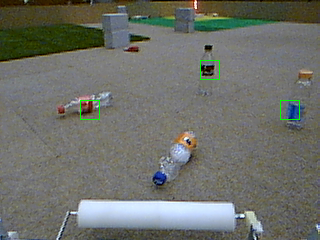
\includegraphics[width=0.45\textwidth]{figures/009.png}}
\hfill
\subfigure{
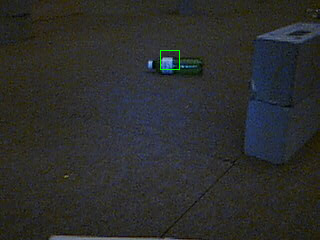
\includegraphics[width=0.45\textwidth]{figures/011.png}}
\label{fig:bottles1}
\caption{Bottle detection at different lightning conditions.}
\end{figure}


\subsubsection{Generated Data}
Output data generated from the above vision algorithms is collected in an object of type
\texttt{VisionMeasure} and handed to the \texttt{Brain}. It contains $x-$ and $y-$coordinates
in pixels, where $y=0$ is the bottom pixel row and $x=0$ is the horizontal center of the
image. There is also a vector of potential bottles with their respective coordinates,
slope and intersect of a regression line fit to the ten central bars and an error measure
reflecting confidence in the regression line.

Even though we could work with 3D data by calibrating the camera with respect to the
floor and compute distances and lateral offsets in cm, we decided to work with pixel
coordinates. We tried translating pixel coordinates into cm by measuring the field of view
of the camera and using the results for linear interpolation. However, this is eventually
only a scaling factor that can easier be taken care of when using the vision data. Hence,
we decided to transmit raw pixel measures and adjust accordingly in the control algorithm.

\subsection{Partial Results}
The terrain segmentation worked very well in most cases. Strong intensity changes on grass
produced poor segmentations. Dimming the ceiling light helped to avoid this. 
Our bottle detection had many false positives since it was very responsive to edges in
general. Rocks formed a particular problem. Taking into account the information
about terrain transitions might have helped to avoid these false positives since the 
rock barrier was detectable without any problems. However, this feature could not 
be added in time before the competition. 

Another problem came up during the competition. Our robot dropped off its bottle 
outside the recycling area due to a constant false positive beacon in the audience. 
High image intensities with a matching width for the top-hat filter.
It was the same place in both cases.
This means that the threshold was chosen too loosely and we could have avoided it.

\section{Control Algorithm}
At the moment our robot is a Braitenberg vehicle, meaning that depending on the type
of reading it receives steers its wheels toward or away from the perceived object.
Terrain classification as well as positions of obstacles and bottles detected through
vision will be added to guide the robot. Special behaviors as picking up a bottle,
returning home to the recycling station or releasing loaded bottles are planned.

In order to control the robot's locomotion a finite state machine has been developed .
In such a system to each state is associated a particular behavior of the robot that is triggered according to some predefined conditions.
The chosen states for our robot are shown in figure \ref{fig:FSM}

\begin{figure}
\centering
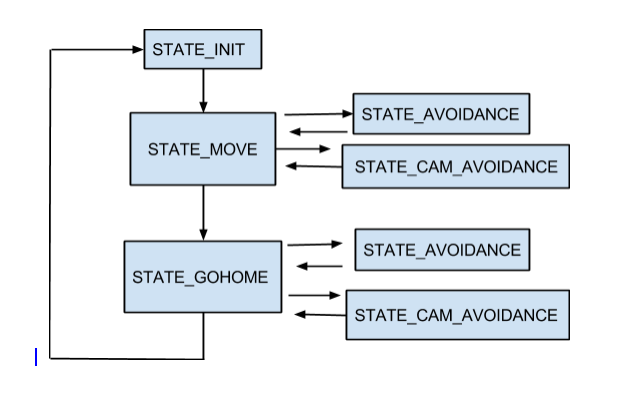
\includegraphics[width=0.8\textwidth]{FSM.png}
\caption{Finite State Machine of the robot.}
\label{fig:FSM}
\end{figure}

At the beginning the robot is the STATE INIT. In this state the robot is initialized, meaning that is checked if the back-door for the bottles release is properly closed and if the brush is moving.
After that the robot is directly moved to the STATE MOVE.
This state represents the default behavior of the robot if no obstacles or changes of zone are detected.
The robot simply moves straight ahead looking for bottles with the camera and, if it detects one of them, it steers toward the bottle in order to grasp it.
Once the bottle has been grasped, it is lifted up thanks to an IR sensor placed within the elevator and which detects if something is in it.
From this state the robot can pass to others three different behaviors according to some trigger conditions.
First of all, if the robot is within a range of 50 cm from an obstacle, that can be either a brick or a wall it enters the STATE AVOIDANCE.
In this state the speeds for the wheels are computed considering the robot as a Braitenberg's vehicle.
This means that a bias speed is assigned to the wheels and then this value are modified exploiting a reactive architecture based on the IR sensors disposed on the robot.
Each sensor gives a value of the distance of the obstacles around the robot and afterwards this value is subtracted to 80 cm (maximum range of the IR sensor) in order to obtain a value that is bigger the closer an obstacle is to the robot. These values are then multiplied for weights properly chosen to conferee a smooth behavior to the robot while avoiding obstacles and modify the bias speeds to allow the robot to avoid having an impact with the brick or the wall.
Being the IR disposed in a symmetric way around the robot, in order to deal with the case in which the robot meets an obstacle perpendicular to it, a safety maneuver has been implemented consisting in making the robot drive backwards and turn of a small angle. This maneuver is activated when both the front IR sensors return a value of distance between a certain threshold that has been chosen of 50 cm.
After the robot has successfully avoided a possible impact it returns in STATE MOVE if the returned values from the sensors are bigger of a disable threshold different from the enable one. The two threshold are different otherwise the robot would just continuously switch between the two states getting stuck in its current location in the arena.
From the STATE MOVE the robot can also switch to the STATE CAM AVOIDANCE.
This state has as objective to allow the robot to identify a change of zone in the arena and avoid crossing it.
This has been done because, even though the robot is capable to cross all the passages areas, in case of failure of the procedure to lift up the robot's elevator the robot would simply risk to break part of its structure. As a consequence it has been chosen to avoid the bonus zones during the competition.
This state exploits the information coming from the camera and if a change in the appearance of the terrain is detected a safety maneuver like the one described before is performed.
Finally the robot can pass from STATE MOVE to STATE GO HOME in order to bring the bottles to the reserved recycling area exploiting the information coming from the compass and then come back to the STATE MOVE.
To avoid an impact during this process, from this state as well is possible for the robot to switch to the two states STATE AVOIDANCE and STATE CAM AVOIDANCE.



   % (\chapter{})
%\cleardoublepage
%%%%%%%%%%%%%%%%%%%%%%%%%%%%%%%%%%%%%%%%%%%%%%%%%%%%%%%%%%%%%%%%%%%%%%%%%%%%%%%%
%
%   Semester project, fall term 2014
%   Author: Jakob Ehrl, born 01/24/91
%   Study program: Computer science, MA 1
%   
%   Professor Dr. Francesco Mondada
%   Assistant: Dr. Stefan Witwicki
%
%%%%%%%%%%%%%%%%%%%%%%%%%%%%%%%%%%%%%%%%%%%%%%%%%%%%%%%%%%%%%%%%%%%%%%%%%%%%%%%%%

\chapter{Schematics and Implementation}

In this section is described the connection between the different modules, voltage sources, and the signal cables.

\section{Modules connection}

The main modules are connected together, with a central processing brain, the Odroid-C1.

\begin{figure}[H]
  \centering
  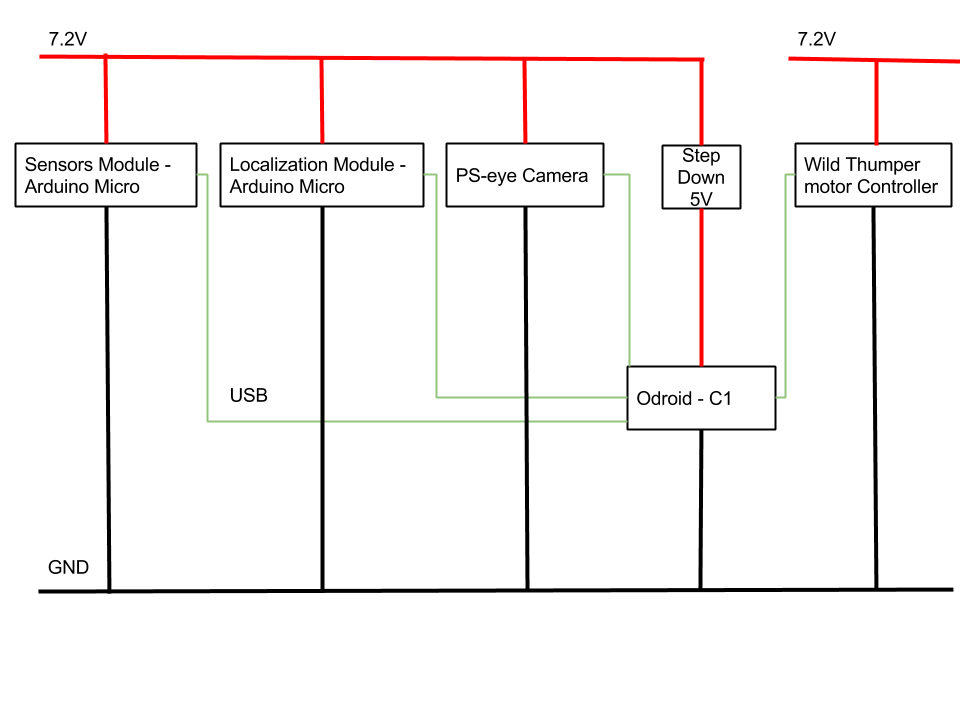
\includegraphics[width=0.8\textwidth]{GlobalConnection.png}
  \caption{The Global abstract connection between the different modules.}
\label{fig:GlobalConnection}
\end{figure}

In the Figure \ref{fig:GlobalConnection} above, is represented the connection diagram between the main modules. As it can be observed, the communication connections between these modules are all USB ( green wire) . This will reduce the number of cables, and ease the communication, as it is an asynchronous protocol, which is widely used and very documented for the arduinos and odroid.\\

Everything is supplied by two battery packs of 7.2 Volts, but have a common ground. The reason for decoupling the wild thumper power supply from the rest comes from the high demand in current required for the motors. This current flow can (if higher than the 10 A of the fuse) burn the fuse for in the power rack. Another reason is that the motors draw much current (2.2 Amps per motor at stall) and if the odroid is connected to the same battery it can happen that the current instability will cause the odroid to fail.

The odroid is connected to a step down voltage regulator, because it needs a stable 5 volts power supply to function correctly.

\section{Sensor Module}

The sensors module, as described in it's respective section, is connected to all the range sensors in the robot. It can also control the brush motor and the Dynamixel smart Servo. An other feature is to read the current that is flowing through the brush motor.

\begin{figure}[H]
  \centering
  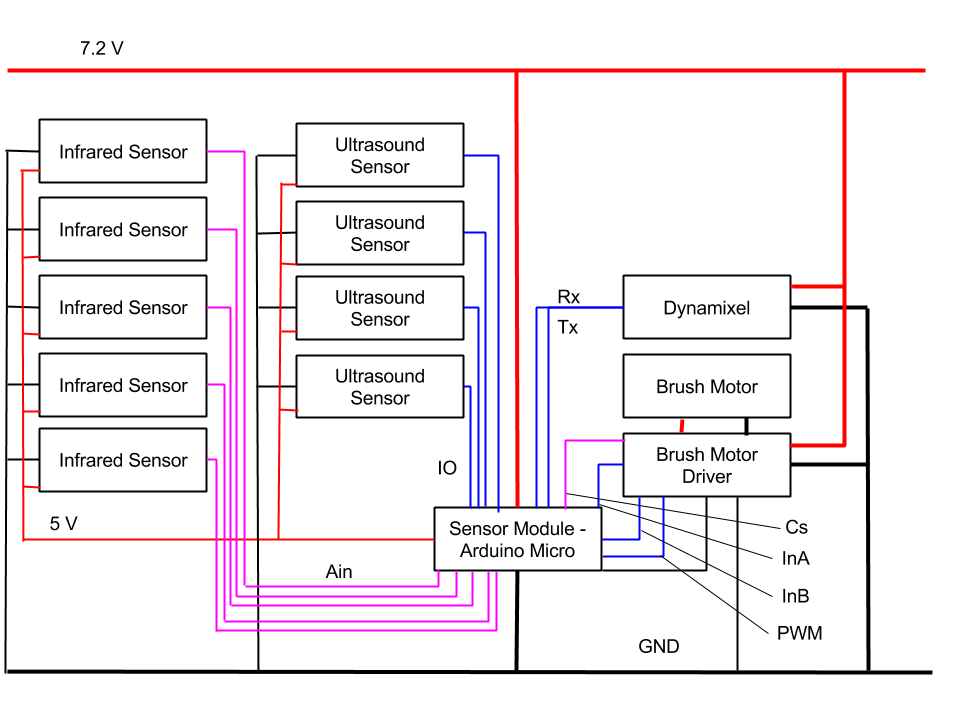
\includegraphics[width=0.8\textwidth]{Arduino1Connection.png}
  \caption{The Sensors module, and it's connections.}
\label{fig:ard1connection}
\end{figure}

As it can be seen in Figure \ref{fig:ard1connection} above, the sensors module is connected to many different sensors. With 20 IO pins and 12 Analog input pins, the arduino Micro is also powerful enough to read, interpred, and connect to all those sensors. In purple are all the analog wires, and blue the IO pins. The Cs is a special pin on the motor driver that allows to read the current flowing through the motor. Each 140mV read on this pin corresponds to 1 Amp on the motor. For the dynamixel, as described earlier, the two serial wires are connected together with a resistance in between to simulate a half duplex connection. The ultrasound sensors, as well have both echo and ping pins connected together with a resistance in between, in order to reduce the number of pins used on the arduino micro, and facilitate the connections.\\

The three other IO pins connected to the motor driver are just controls for the motor. The motor driver needs two power supplies. One is for the input logic, 5V, and the other is for the motor output (we used the battery 7.2 V power supply).\\

Figure \ref{fig:ard1connection} was the planned connections, but was not what was used in the end, during the competition, a more accurate figure would be Figure \ref{fig:ard1connection2} seen below, where only infrared sensors were used.

\begin{figure}[H]
  \centering
  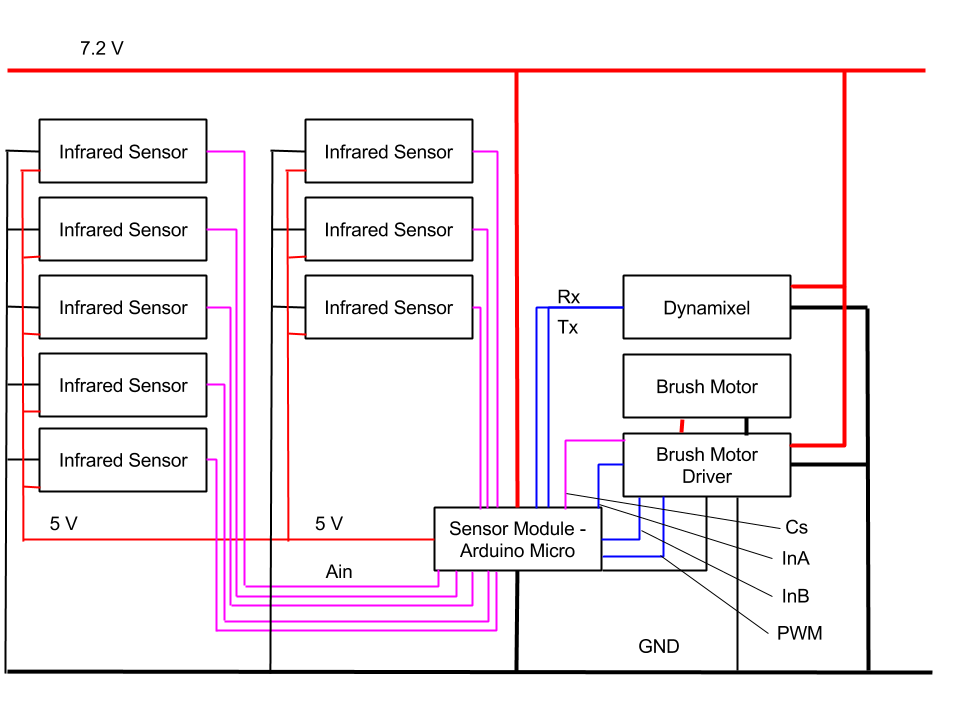
\includegraphics[width=0.8\textwidth]{Arduino1Connection2.png}
  \caption{The Sensors module, and it's connections.}
\label{fig:ard1connection2}
\end{figure}

\section{Localization Module}

The localization module is, as described in the section previously, the module that uses 6 line sensor arrays and a compass to locate the position and yaw of the robot. 

\begin{figure}[H]
  \centering
  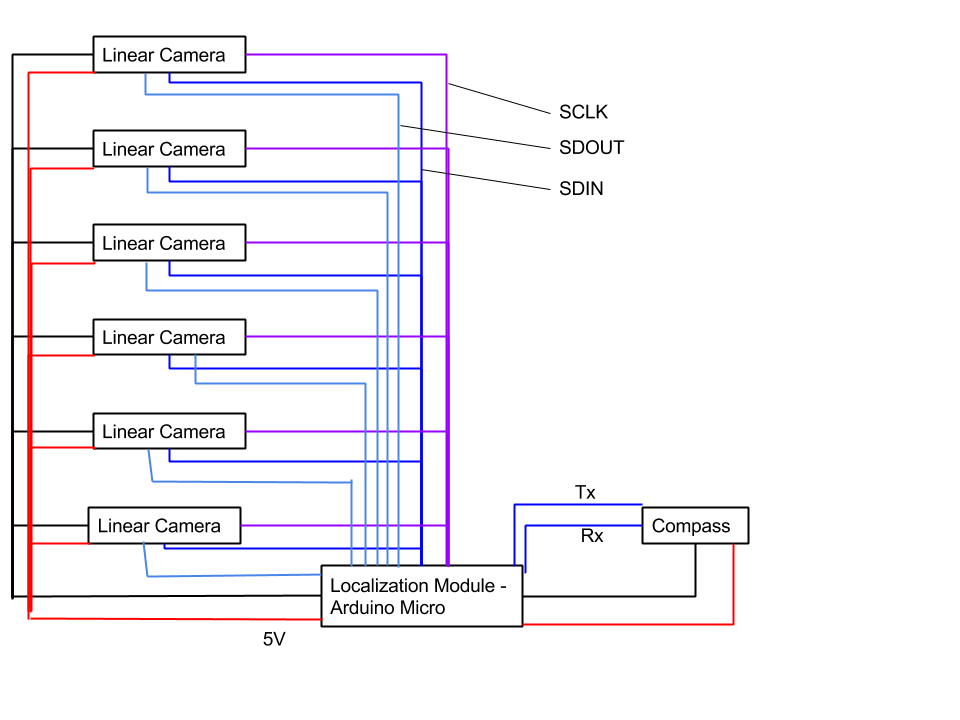
\includegraphics[width=0.8\textwidth]{Arduino2Connection.png}
  \caption{The Localization module, and it's connections.}
\label{fig:ard2connection}
\end{figure}

The connection between the arduino micro and the sensors is shown in the Figure \ref{fig:ard2connection} above. The compass uses a simple serial connection, and the arduino micro has two of them ( USB and serial pins). For the linear cameras, three lines were necessary. SCLK, the clock, can be common between the sensors, since it does not have any effect if no data is transmitted. %The SDIN lines are soldered together as well, XXXXXXXXXXXXXXXXXXXXXXXXXXXXXXXXXXXXXXXX
%XXXXXXXXXXXXXXXXXXXXXXXXXXXXXXXXXXXXXXXXXXX
%XXXXXXXXXXXXXXXXXXXXXXXXXXXXXXXx
%XXXXXXXXXXXXXXXXXXXXXXXXXXXXXXX
%XXXXXXXXXXXXXXXXXXXXXXXXXXXXXXX

\section{Motor driver module}

The motor driver module has very simple connections. The only devices it is controlling are the motors, and the tailgate servo.

\begin{figure}[H]
  \centering
  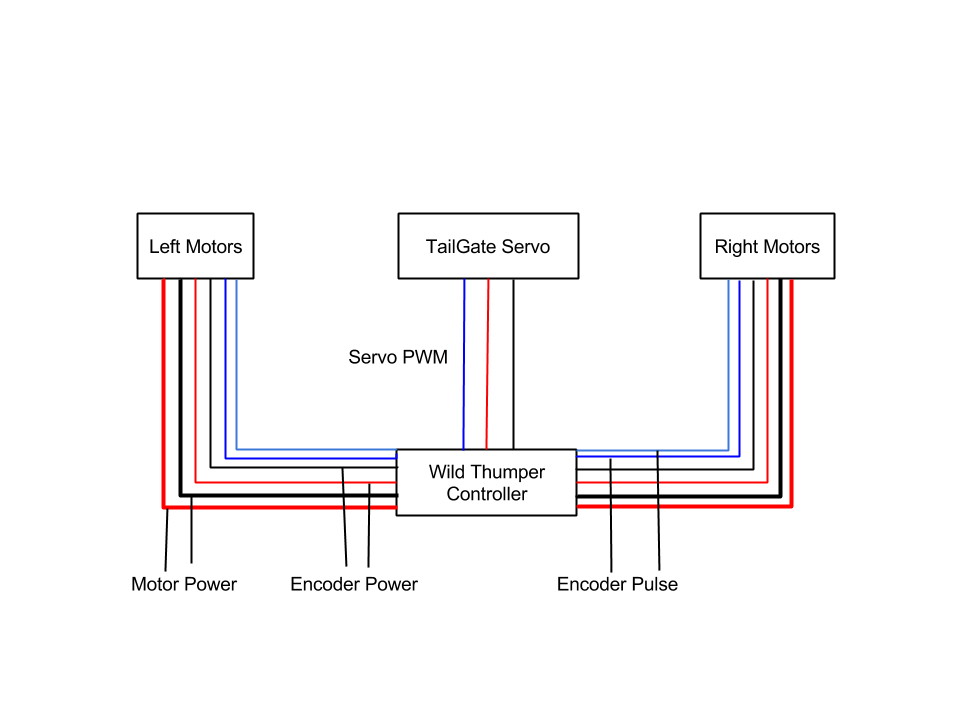
\includegraphics[width=0.8\textwidth]{WildThumperConnection.png}
  \caption{The Motor Driver Module, and it's connections.}
\label{fig:wtconnection}
\end{figure}

Seen in Figure \ref{fig:wtconnection} above is the connection diagram of the wild thumper motor controller. The only signals it is reading are the motor encoders, which allow to estimate a precise speed, and position of the wheels.

%\chapter{Implementation}
%how everything was connected, connectors etc.. battery... 

\chapter{Results}
The robot was the second one in the competition. With 2.5 poits, the robot was able to capture a bottle and nearly bring it back in time. The remote control from a computer allowed us to control manually all the functions of the robot, the wheels, the servos, and the brush, and we were also able to visualize the camera, and see the values of all the different sensors. The robot was able to navigate towards a bottle, to avoid obstacles, and was also able to return home and open the tailgate. However, as many false positives were measured from the camera, the robot sometimes saw beacons, and thus released the bottles. Another feature was area distinction, which allowed the robot to avoid going in dangerous zones, but there, once again, the false positives would make the robot go towars the rocks for instance. As the shovel was close to the ground, the robot sometimes got stuck in between the tiles, under the grass or the rocks. In the beginning it was planned to use two dynamixels, because one was not strong enough to just `hover' the lift above the ground, but since the synchronization of the servos failed, we could only have two states : on the ground or lifted all the way.

\chapter{Conclusion}
Finally, this huge project took a tremendous amount of our time. In order to accomplish a functionnal robot, nearly every day was spend in epfl until midnight, where intense work took place. It was quite sad to obtain a robot that did not manage to bring back more than one bottle at the end, especially considering the amount of work invested in the project. However, all this work allowed us to learn very much on the design, construction and programming of a robot, with all the project phases in between.

\chapter{Annex}

\begin{figure}[H]
  \centering
  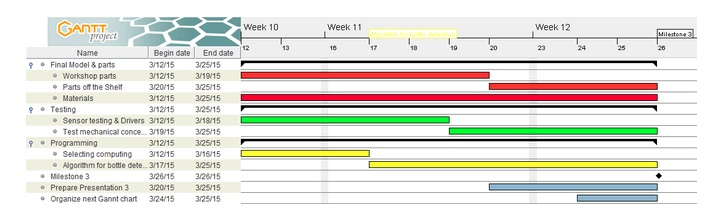
\includegraphics[width=0.8\textwidth]{GanttChart1.jpg}
  \caption{Gannt Chart until the third milestone.}
\label{fig:gannt1}
\end{figure}

\begin{figure}[H]
  \centering
  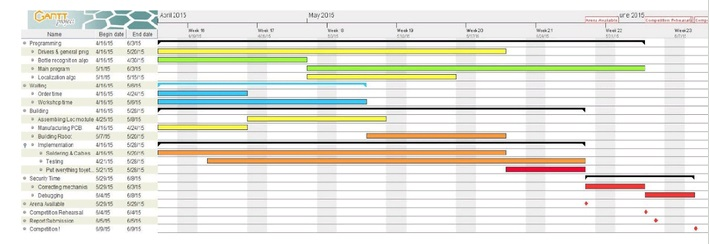
\includegraphics[width=0.8\textwidth]{GanttChart2.jpg}
  \caption{Gannt Chart until the end of the competition.}
\label{fig:gannt2}
\end{figure}

\begin{figure}[H]
  \centering
  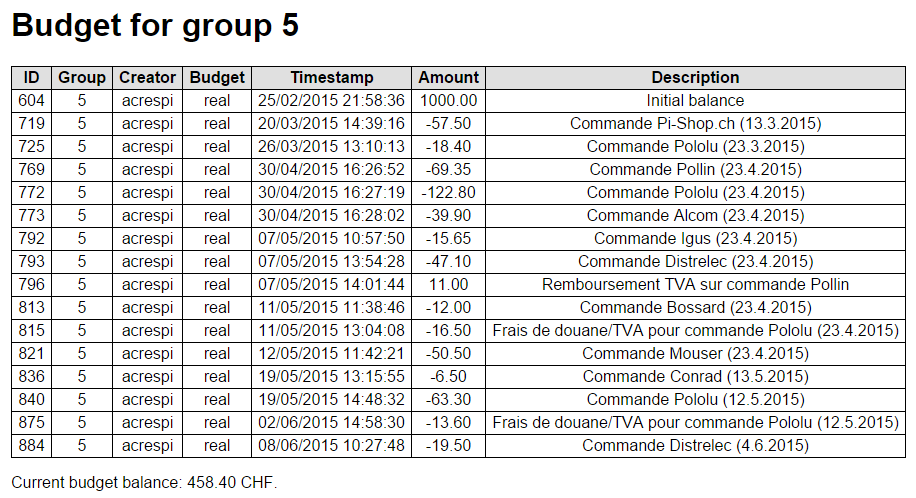
\includegraphics[width=0.8\textwidth]{budgetreal.png}
  \caption{Real budget used for the robot.}
\label{fig:real}
\end{figure}

\begin{figure}[H]
  \centering
  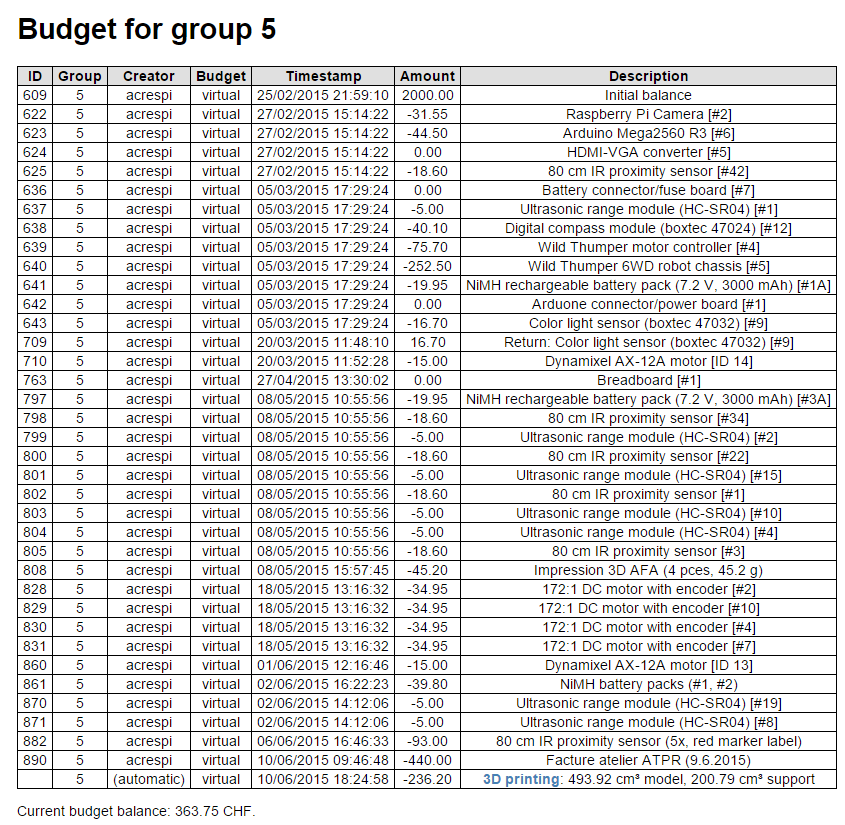
\includegraphics[width=0.8\textwidth]{budgetvirtual.png}
  \caption{Virtual budget used for the robot.}
\label{fig:virtual}
\end{figure}   % (\chapter{})
%\cleardoublepage
%\include{rc08}   % Zusammenfassung (\chapter{Zusammenfassung}  TEXT)
%\cleardoublepage

%\appendix
%\cleardoublepage
%\include{rc09}   % Glossar (\chapter{Glossar}  TEXT)
%\cleardoublepage
%\include{rc10}   % 
%\cleardoublepage
%\include{rc11}   % 
%\cleardoublepage

%%%%%%%%%%%%%%%%%%%%%%%%%%%%%%%%%%%%%%%%%%%%%%%%%%%%%%%%%%%%%%%%%%%%%%%%%%
% Diese Datei nicht veraendern!
%%%%%%%%%%%%%%%%%%%%%%%%%%%%%%%%%%%%%%%%%%%%%%%%%%%%%%%%%%%%%%%%%%%%%%%%%%
\addcontentsline{toc}{chapter}{\listfigurename}
\listoffigures
 % Bilderverzeichnis
%%\cleardoublepage
%%\clearpage
%%%%%%%%%%%%%%%%%%%%%%%%%%%%%%%%%%%%%%%%%%%%%%%%%%%%%%%%%%%%%%%%%%%%%%%%%%
% Diese Datei nicht veraendern!
%%%%%%%%%%%%%%%%%%%%%%%%%%%%%%%%%%%%%%%%%%%%%%%%%%%%%%%%%%%%%%%%%%%%%%%%%%
\addcontentsline{toc}{chapter}{\listtablename}
\listoftables
 % Tabellenverzeichnis
%%\cleardoublepage
%%\clearpage
%%%%%%%%%%%%%%%%%%%%%%%%%%%%%%%%%%%%%%%%%%%%%%%%%%%%%%%%%%%%%%%%%%%%%%%%%%
% Diese Datei nicht veraendern!
%%%%%%%%%%%%%%%%%%%%%%%%%%%%%%%%%%%%%%%%%%%%%%%%%%%%%%%%%%%%%%%%%%%%%%%%%%
\addcontentsline{toc}{chapter}{\bibname}
\bibliography{ml}
 % Literaturverzeichnis

\end{document}
